\documentclass[12pt,twoside]{report}
\usepackage{setspace}
\usepackage{amsmath}
\usepackage[pdftex]{graphicx}
\usepackage{suthesis-2e}
\usepackage{hyperref}
\usepackage{multirow}
\usepackage{todonotes}
\usepackage{tikz}
\usepackage{gantt}
\usepackage{listings}
\usepackage{xcolor}
%\lstset{language=C,
%           basicstyle=\ttfamily\tiny,
%           backgroundcolor=\color{black!5}, % set backgroundcolor
%           keywordstyle=\color{blue}\ttfamily,
%           stringstyle=\color{red}\ttfamily,
%           commentstyle=\color{green}\ttfamily,
%          breaklines=true
%          }

\usepackage{calc}
\usepackage{array}
\usepackage{rotating}
\usepackage{url}
\usepackage{pgf,tikz}
\usetikzlibrary{snakes,arrows,shapes}
\usepackage{adjustbox}
\usepackage{dot2texi}
\usepackage[normal]{subfigure}
\usepackage{multirow}
\usepackage{todonotes}
\usepackage{tikz}
\usepackage{xcolor}
\usepackage{pgfplots, pgfplotstable}
\usepackage{amsmath}
\usepackage{pgf,tikz}
\usetikzlibrary{snakes,arrows,shapes}

\usepackage{amsmath}
\usepackage{mdwlist}
\usepackage{xcolor}
\usepackage{adjustbox}
\usepackage{dot2texi}
\usepackage{fancyhdr}



\usepackage{pgfplots, pgfplotstable}
\usepackage{amsmath}
\makeatletter
\newif\if@restonecol
\makeatother
\let\algorithm\relax
\let\endalgorithm\relax
\usepackage[ruled]{algorithm2e}
\usepackage{multirow}
\usepackage[center]{caption}
\usepackage{xcolor}
\usepackage{tikz}
\usepackage{calc}
\def\checkmark{\tikz\fill[scale=0.4](0,.35) -- (.25,0) -- (1,.7) -- (.25,.15) -- cycle;} 
\def\scalecheck{\resizebox{\widthof{\checkmark}*\ratio{\widthof{x}}{\widthof{\normalsize x}}}{!}{\checkmark}}
\usetikzlibrary{arrows,backgrounds}
\usetikzlibrary{arrows,automata,calc,shapes,positioning,shadows,trees}

\pgfplotsset{compat=newest}


\tikzset{
  basic/.style  = {draw, text width=2cm, font=\sffamily, rectangle},
  root/.style   = {basic, rounded corners=2pt, thin, align=center,
                   fill=white!90},
  level 2/.style = {basic, rounded corners=6pt, thin,align=center, fill=white!90,
                   text width=8em},
  level 3/.style = {basic, thin, align=left, fill=white!90, text width=6.5em}
}


\usepackage{acro}

% class `abbrev': abbreviations:
\DeclareAcronym{FHE}{
	short = FHE ,
	long  = Fully Homomorphic Encryption ,
	class = abbrev
}
\DeclareAcronym{FFT}{
	short = FFT ,
	long  = Fast Fourier Transform ,
	class = abbrev
}
\DeclareAcronym{FFTW}{
	short = FFTW ,
	long  = Fast Fourier Transform in the West ,
	class = abbrev
}
\DeclareAcronym{FHEW}{
	short = FHEW ,
	long  = Fully Homomorphic Encryption Library ,
	class = abbrev
}
\DeclareAcronym{NTT}{
	short = NTT ,
	long  = Number Theoretic Transform,
	class = abbrev
}
\DeclareAcronym{FPGA}{
	short = FPGA ,
	long  = Field Programmable Gate Array ,
	class = abbrev
}
\DeclareAcronym{GPU}{
	short = GPU ,
	long  = Graphics Processing Unit ,
	class = abbrev
}
\DeclareAcronym{CPU}{
	short = CPU ,
	long  =  Central Processing Unit ,
	class = abbrev
}
\DeclareAcronym{HLS}{
	short = HLS ,
	long  = High Level Synthesis,
	class = abbrev
}
\DeclareAcronym{OpenCV}{
	short = OpenCV ,
	long  = Open Source Computer Vision,
	class = abbrev
}
\DeclareAcronym{CNN}{
	short = CNN ,
	long  = Convolutional Neural Network,
	class = abbrev
}
\DeclareAcronym{2D}{
	short = 2D ,
	long  = Two Dimensional ,
	class = abbrev
}
\DeclareAcronym{MNIST}{
	short = MNIST ,
	long  = Modified National Institute of Standards and Technology,
	class = abbrev
}
\DeclareAcronym{LFHE}{
  short = LFHE ,
  long  = Levelled Fully Homomorphic Encryption ,
  class = abbrev
}
\DeclareAcronym{LWE}{
  short = LWE ,
  long  =Learning With Errors ,
  class = abbrev
}
\DeclareAcronym{RTL}{
  short = RTL ,
  long  = Register Transistor Logic,
  class = abbrev
}

\DeclareAcronym{IP Core}{
  short = IP Core ,
  long  = Intellectual Property Core ,
  class = abbrev
}

\usepackage{color}
\definecolor{lightgray}{rgb}{0.95, 0.95, 0.95}
\definecolor{darkgray}{rgb}{0.5, 0.5, 0.5}
\definecolor{purple}{rgb}{0.65, 0.12, 0.82}

\definecolor{ocherCode}{rgb}{1, 0.5, 0} % #FF7F00 -> rgb(239, 169, 0)
\definecolor{blueCode}{rgb}{0, 0, 0.93} % #0000EE -> rgb(0, 0, 238)
\definecolor{greenCode}{rgb}{0, 0.6, 0} % #009900 -> rgb(0, 153, 0) 
\usepackage{upquote}
\usepackage{listings}
\makeatletter
%\lstdefinelanguage{HTML5}{
%	sensitive=true,
%	keywords={%
%		% JavaScript
%		typeof, new, true, false, catch, function, return, null, catch, switch, var, if, in, while, do, else, case, break,
%		% HTML
%		html, title, meta, style, head, body, script, canvas,
%		% CSS
%		border:, transform:, -moz-transform:, transition-duration:, transition-property:,
%		transition-timing-function:
%	},
%	% http://texblog.org/tag/otherkeywords/
%	otherkeywords={<, >, \/},   
%	ndkeywords={class, export, boolean, throw, implements, import, this},   
%	comment=[l]{//},
%	% morecomment=[s][keywordstyle]{<}{>},  
%	morecomment=[s]{/*}{*/},
%	morecomment=[s]{<!}{>},
%	morestring=[b]',
%	morestring=[b]",    
%	alsoletter={-},
%	alsodigit={:}
%}


\usepackage{float}
\usepackage{booktabs}
\usepackage{array}
\usepackage{caption}
%\usepackage{subcaption}
\usepackage{multirow}
\usepackage{rotating}
\usepackage{url}
\usepackage{tikz}
%\usetikzlibrary{dsp,chains}
\usepackage{pgf,tikz}
\usetikzlibrary{calc,arrows}
\usepackage{amsmath}
%\usepackage{minted}
%\usepackage{titlesec}
%\usepackage{ulem}
%\usepackage{subfigure}
%\usepackage{subcaption}
\setcounter{secnumdepth}{3}
\setcounter{tocdepth}{2}
%\setcounter{secnumdepth}{4}
%\setcounter{tocdepth}{4}
\renewcommand{\topfraction}{0.9}	% max fraction of floats at top
\renewcommand{\bottomfraction}{0.8}	% max fraction of floats at bottom
%Parameters for TEXT pages (not float pages):
\setcounter{topnumber}{2}
\setcounter{bottomnumber}{2}
\setcounter{totalnumber}{4}     % 2 may work better
\setcounter{dbltopnumber}{2}    % for 2-column pages
\renewcommand{\dbltopfraction}{0.9}	% fit big float above 2-col. text
\renewcommand{\textfraction}{0.07}	% allow minimal text w. figs
%Parameters for FLOAT pages (not text pages):
\renewcommand{\floatpagefraction}{0.7}	% require fuller float pages
%N.B.: floatpagefraction MUST be less than topfraction !!
\renewcommand{\dblfloatpagefraction}{0.7}	% require fuller float pages
%remember to use [htp] or [htpb] for placement

\newenvironment{packed_enum}{
\begin{enumerate}
  \setlength{\itemsep}{1pt}
  \setlength{\parskip}{0pt}
  \setlength{\parsep}{0pt}
}{\end{enumerate}}

\pagestyle{fancy}
\fancyhead{}
\fancyfoot{}

\fancyhead[RO,LE] {\thepage}
\fancyhead[RE] {\leftmark}
\fancyhead[LO]{\rightmark}
\renewcommand{\headrulewidth}{0pt}
\begin{document}


\begin{titlepage}
\begin{center}
{\LARGE {NANYANG TECHNOLOGICAL UNIVERSITY}}
\begin{figure}[!t]
\centering
\includegraphics[width= 8 cm]{figures/ntulogo.pdf}
\end{figure} 
\vspace*{0.7in}
{\large EXPLORING THE ARITHMETIC OF COMPUTATIONALLY INTENSE APPLICATIONS ON HETEROGENEOUS PLATFORMS}
\par
\vspace{0.4 in}
{\large by\\}
\vspace{0.2 in}
{\large DEEPSHIKHA

(G1601338G)}
\vspace{0.1 in}
\par
\vfill
A Dissertation Submitted in partial fulfillment of \\ the requirements for the degree of \\ Master of Science in Embedded Systems
\par
\vspace{0.4in}
Supervised by\\
%\par
\vspace{0.1in}
{\large Assoc. Prof. Douglas L. Maskell \\}
\par
\vspace{0.15in}
July 2016
\end{center}
\end{titlepage}
%\onehalfspacing
\pagenumbering{roman}
\tableofcontents
\listoffigures
\listoftables
\renewcommand{\lstlistlistingname}{List of Source Codes}
\lstlistoflistings

\chapter*{Abbreviations}
\begin{table}[h]
\begin{tabular}{m{3cm} m{15cm}}
\textbf{FHE} & Fully Homomorphic Encryption\\
\vspace{0.25cm}
\textbf{FFT} &  Fast Fourier Transform\\
\vspace{0.25cm}
\textbf{FFTW} & Fast Fourier Transform in the West\\
\vspace{0.25cm}
\textbf{FHEW} & Fully Homomorphic Encryption Library\\
\vspace{0.25cm}
\textbf{NTT} & Number Theoretic Transform\\
\vspace{0.25cm}
\textbf{FPGA} & Field Programmable Gate Array\\
\vspace{0.25cm}
\textbf{GPU} & Graphics Processing Unit\\
\vspace{0.25cm}
\textbf{CPU} & Central Processing Unit\\
\vspace{0.25cm}
\textbf{HLS} & High Level Synthesis\\
\vspace{0.25cm}
\textbf{OpenCV} & Open Source Computer Vision\\
\vspace{0.25cm}
\textbf{CNN} & Convolutional Neural Network\\
\vspace{0.25cm}
\textbf{2D} & Two Dimensional\\
\vspace{0.25cm}
\textbf{MNIST} & Modified National Institute of Standards and Technology\\
\vspace{0.25cm}
\textbf{LFHE} & Levelled Fully Homomorphic Encryption\\
\vspace{0.25cm}
\textbf{LWE}  & Learning With Errors\\
\vspace{0.25cm}
\textbf{RTL}  & Register Transistor Logic\\
\vspace{0.25cm}
\textbf{IP Core}  &  Intellectual Property Core\\
\end{tabular}
\end{table}
 
\begin{abstract}
	
Homogeneous computing platforms, specifically multi-core CPUs spend most of the execution time on non-computational tasks (handling data movements, fetching and decoding instructions), with a lot of power spent on non-computational units. The strong need for increased computational performance has led to the use of heterogeneous computing platforms, with graphics processing units (GPUs) and massively parallel processor arrays(MPPAs) acting as co-processors for arithmetic intensive data-parallel workloads. However energy efficiency remains a major concern.
For more than a decade, researchers have shown that FPGAs can accelerate a wide variety of compute-intensive applications in an energy-efficient manner, in some cases by several orders of magnitude compared to state of-the-art general purpose processors. This is due to highly customized hardware implementation designed specifically for the compute kernels which basically require extensive analysis (in terms of arithmetic complexity) and the performance demands of the application. For example, researchers have shown that implementation of convolutional layers of deep neural networks does not need to rely on expensive floating point hardware resources and can be handled using low precision fixed point hardware resources leading to more efficient execution in terms of area, latency and power. 
However, changing the arithmetic of an application may have adverse affects on the accuracy because of the precision loss by changing the data types. This report aims to explore these trade-offs by analyzing two compute-intensive applications. The first one is Fully Homomorphic Encryption (FHE) and the second one is Convolution Neural Network (CNN) used for digit classification problem.
 
\end{abstract}



\pagenumbering{arabic}

\chapter*{Acknowledgment} 
\label{ch0_Acknowledgement}
I would like to express my sincere thanks to Assoc. Prof. Dr. Douglas Leslie Maskell for providing me the opportunity to work on this project. I would like to thank him for his encouragement and support.
My deepest gratitude to Dr. Abhishek Kumar Jain for his guidance and persistent help on different aspects of my work . I am really thankful to him for his motivation and constant mentor ship throughout the course of this dissertation.
I would also like to thank my classmate Swarna, for helping and supporting me at all times.
Thanks to Mr. Jeremiah Chua for his help with the lab resources.
Last but not the least I would like to express my gratitude and reverence to my parents for being the strength of my life.

%\ac{ICON}
%\ac{JTAG
%\ac{ADC}
%\ac{MSps}
% 
%\ac{MBps}
% 
%\ac{Mbps}
% 
%\ac{KSps}
%  
%\ac{KBps}
% 
%\ac{Kbps}

%\ac{BSP}


%\ac{RTL}
%\ac{SDK}




\chapter{Introduction}
\label{ch1_introduction}
\section{Motivation}

Technology scaling has led to implementation of larger circuits on a single chip. At the same time, the saturation of frequency scaling has led to exploration of parallelism by running multiple applications on hardware to gain speedup. These days both software and hardware solutions e.g. Desktops, Laptops, General Purpose Processors are supplied with multiple processors or hardware accelerators which consist of multiple small execution units to facilitate parallelism for reducing the computation time of applications. 

\vspace{0.25cm}
 Various hardware accelerators are based on GPU's, Cell Processors or FPGA's. At times software execution of certain applications takes more time than the hardware execution. Depending on the algorithm,specific accelerators may perform better than other accelerators. Hence running an algorithm efficiently is ideally a mapping an algorithm to architecture problem.
\begin{figure}[!h]
\centering
\includegraphics[scale=0.65]{figures/performance.png}
\caption{Performance Vs. Flexibility for Different Architectures.(Source \ref{architechture})}
\label{fig:Performance}
\end{figure}
\vspace{0.25cm}
 However there are certain trade-offs that need to be taken into account. e.g as given in figure \ref{fig:Performance} ASIC give the best performance in terms of time and power, but it offers less flexibility. On the other hand Microprocessors offer flexibility for programming while compromising on performance. FPGA offer hardware reconfigurablility, so it is preferred for customized designs.

\vspace{0.25cm}
 Most of the applications in present environment are computation intensive and require real time processing.For such applications performance can be enhanced by using hardware software co-design, wherein a part of an algorithm can be offloaded to hardware accelerator, with the help of bus architectures. The challenge in this process is to identify the portions of the applications which will give speedup on hardware under resource constraints. Usually the identification is based on the execution times or computation requirements.  
\begin{figure}[!h]
\centering
\includegraphics[scale=0.65]{figures/DSE.png}
\caption{Design Space Exploration for Algorithm Acceleration.(Source \ref{architechture})}
\label{fig:DSE}
\end{figure}
\vspace{0.25cm}

 When hardware accelerators are used, certain modifications specific to the accelerator help in getting performance benefits. e.g. in FPGA, datatypes and bit widths have significant impact on the performance. e.g. Single precision floating point datatype consumes lesser number of resources than double precision floating point datatype. Similarly fixed point computation units require lesser number of resources than floating point computation units, which can be used to increase number of concurrent executions of an algorithm and hence increasing in parallelism which may help to gain speedup. However these modifications directly impact the correctness of the algorithm. 
 
\vspace{0.25cm}
In this report, the first two steps of the design space exploration for algorithm acceleration as given in figure \ref{fig:DSE} are explored for two algorithms:FHEW and Deep Neural Network. The focus is on identification of compute intensive portions of the algorithm to be accelerated on hardware by thoroughly studying the functionality and the modification of underlying arithmetic for performance benefits. Implementation of compute intensive portion for HDL, and the gain estimation in terms of area and latency is also studied using the tool Vivado HLS.


\section{Contribution}
The main contributions can be summarized as follows:

\vspace{0.25cm}
\textbf{Fully Homomorphic Encryption (FHEW) Algorithm}
\begin{itemize}
\item
Understanding the algorithm and the existing implementation to identify the computation intensive modules of the algorithm. 
\item
Experiments of modifications of the existing library from double precision float to single precision float.
\item
Bottom-up analysis of Fast Fourier Transform, starting from a single butterfly unit, to yield a resource optimized implementation of 1024-point FFT, for efficient implementation of FHEW on hardware.
\end{itemize}

\textbf{Deep Neural Network}
\begin{itemize}
\item
Understanding the fixed point arithmetic and writing C scripts to implement fixed point mathematics.
\item
Modification of the existing implementation to support fixed point arithmetic.
\item
Analyzing the inaccuracy that can be tolerated in the algorithm, by varying the number of bits used for fixed point Q format. 
\item
Estimating the improvement in area and latency by implementing the computation intensive module for hardware using Vivado HLS. 
\end{itemize}

\section{Organization}

The remainder of the report is organized as follows:

\vspace{0.25cm}
Chapter \ref{Chapter2} gives background information on Fully Homomorphic Encryption Algorithm(FHEW), Deep Neural Network and Basics of floating point and fixed point arithmetic.\par
\vspace{0.25cm}
Chapter \ref{Chapter3} presents the modification of arithmetic of FHEW from double precision floating point to single precision floating point and a thorough analysis of the results.\par
\vspace{0.25cm}
Chapter \ref{Chapter4} discusses the implementation of an area optimized 1024 point FFT (Fast Fourier Transform) on Vivado HLS,starting from the analysis of smallest butterfly compute unit.\par
\vspace{0.25cm}
Chapter \ref{Chapter5}, discusses the existing implementation of lenet model for classification of MNIST dataset.It also discusses the mathematics of fixed point briefly and a library \textit{Libfi} which is used to integrate fixed point mathematics with the above mentioned implementation of Lenet model. It also tabulates the results of the modification on accuracy, area and latency.  \par
\vspace{0.25cm}
Chapter \ref{Chapter6} summarizes the results of the analysis and suggests areas for future work.








\chapter{Background}
\label{Chapter2}
The two computationally intense algorithms, highlighted in this report involve an encryption algorithm and a neural network. Analyzing the underlying arithmetic require a detailed knowledge of the underlying concepts and basis of the algorithm. 
A thorough understanding of the operations and number representations specific to the arithmetic is also a prerequisite to manipulate an algorithm's underlying mathematics. 
In this chapter the basics of encryption algorithm, neural networks, number representations and fixed point mathematics is discussed in detail.

\section{Cryptography}
Cryptography was invented with an intent of secure communication. It prevents unauthorized users to access and modify the data, ensuring reliable communication by avoiding data corruption. It also prevents information loss. Various applications involving cryptography include military applications, smart cards, passwords etc.
Two main processes involved in cryptography are encryption and decryption:

\begin{itemize}
\label{Encryption}
\item \textbf{Encryption} is a process of converting the data in a complicated form such that it is not readable by unintended users. Encryption is performed on a data known as plaintext to generate another form of data which is encrypted known as ciphertext.
\label{Decryption}
\item \textbf{Decryption} is a process of converting the data in a readable form from an unintelligible form only by the intended users.
\end{itemize}

Modern cryptographical algorithms are based on computationally hard mathematical operations and computer science practices, and hence they require faster computing technology for efficiency.
Encryption is of two types:
\begin{enumerate}
\item \textbf{Symmetric Encryption:} In this type of encryption scheme, a single key is used for encryption as well as decryption.
\item \textbf{Asymmetric Encryption:} In this type of encryption scheme two different keys are used. Public key is used to encrypt a piece of information and a secret key is used for decryption. The public key is usually available publicly, whereas the secret key is only provided to the intended users. Asymmetric encryption is more computationally intense as compared to symmetric encryption and hence requires more processing power and at times is slower. 

\begin{figure}[H]
\centering
\includegraphics[scale=0.8]{figures/asym.PNG}
\caption{Asymmetric Encryption and Decryption}
\label{fig:Asymmetric Encryption}
\end{figure}

\end{enumerate}
With the advancement of cloud based applications which at times deal with sensitive information, it is required to encrypt the data prior to storing on cloud. Homomorphic encryption is devised to make  use of the computational power of cloud.
\subsection{Homomorphic Encryption}
The basic idea of homomorphic encryption scheme is to delegate the processing of data to the cloud without giving access to it.

\vspace{0.25cm}
\begin{figure}[!h]
\centering
\includegraphics[scale=0.7]{figures/Capture1.PNG}
\caption{Conventional Encryption}
\label{fig:Conventional Encryption}
\end{figure}
\noindent Let us say a user has  a set of confidential data and he or she wants to process that data on a cloud or server. The normal procedure would be as specified in the figure \ref{fig:Conventional Encryption} wherein the user encrypts the data to be processed and sends it on to the server. At the server end, the data is decrypted using the secret key, the computation is performed and the resulting data is again encrypted and sent back to the user, which the user can decrypt to get back the end result of the computation.
%figure
\begin{figure}[H]
\centering
\includegraphics[scale=0.7]{figures/Capture.PNG}
\caption{Homomorphic Encryption}
\label{fig:Homomorphic Encryption}
\end{figure}

%http://www.americanscientist.org/libraries/documents/201286159329266-2012-09CompSciHayes.pdf
\vspace{0.25cm}
However if the user wants a secure application, wherein the data is not decrypted even at the server, homomorphic encryption can be used. It allows performing computations over encrypted data, resulting in a data which when decrypted gives back an output which the same as the original result after performing the computation on plain text (Refer figure \ref{fig:Homomorphic Encryption}).

\subsubsection{Steps involved in Homomorphic Encryption} \label{steps}
Typically any encryption scheme involves three algorithms:
\begin{enumerate}

    \item 
    \textbf{Keygen:} Here in a L bit-length key is generated using an algorithm. In case of symmetric encryption schemes, a single key is generated for both encryption and decryption. In case of asymmetric encryption scheme, two keys are generated: public key(pk) which is available to all users and is used for encryption of message and a secret key (sk) which is used for decryption and is available only to the intended users.
   
   \item
    \textbf{Encryption:} As specified in \ref{Encryption} encryption is a process of encoding a message using a key to form a ciphertext.
   
    \item
    \textbf{Decryption:} As specified in \ref{Decryption} decryption is a process of decoding a ciphertext back to original readable form using a key.
   
   \noindent A homomorphic encryption has an additional algorithm involved in addition to the above three.
   
    \item 
     \textbf{Evaluate:} Evaluate is associated with a set of functions, for which the computation is supported by the scheme. A function f on a set of numbers (n\textsubscript{1},n\textsubscript{2},......,n\textsubscript{t}) is intended to be performed, where (c\textsubscript{1},c\textsubscript{2},......,c\textsubscript{t}) represent the encryption of given numbers using a public key (pk) under the homomorphic encryption scheme. The result of evaluate algorithm 'c' which is applied on (c\textsubscript{1},c\textsubscript{2},......,c\textsubscript{t}) to perform the function f is the encryption of f(n\textsubscript{1},n\textsubscript{2},......,n\textsubscript{t}) under the public key (pk). In other words, if we decrypt the result of evaluate algorithm with the corresponding secret key we get back f(n\textsubscript{1},n\textsubscript{2},......,n\textsubscript{t}).
     
     \noindent The efficiency of evaluation function depends primarily on the size of ciphertexts and the function being computed.
\end{enumerate}
     The above works only for a set of functions which are allowed or supported by the encryption scheme. 
    
\subsubsection{Issues with Homomorphic Encryption Scheme} \label{limitations}
\begin{itemize}
\item
\textbf{Semantic Security:} Semantic security refers to the security in terms of the one wayness of encryption algorithm. i.e. There should not be any polynomial time algorithm which can guess the plaintext and private key (pk). To ensure semantic security an encryption scheme must present multiple encryptions of the same plaintext given a public key. However if there is always a one to one mapping, the scheme cannot be ensured to be secure. So encryption algorithms should be hard enough to be broken by attackers. 
\item 
\textbf{Noise in Ciphertexts:} When a ciphertext is encrypted, a fixed term is added to it to ensure the security of the scheme which is called noise. It may be a small number or some polynomial based on whether the scheme is for integers or polynomials. A ciphertext can be decrypted if and only if the noise is less than a certain maximum value. As certain operations are performed on the ciphertexts in homomorphic encryption, the noise grows. The increase in noise in the final ciphertext is based on the operation and also on the depth of operations.

 \noindent Given the encryption function as $Enc(x)=a\times r+b\times n+x$ where x is the message, r is a random variable, a is the secret key and n is the noise. The decryption can be performed on the above encryption function as: 

 \noindent\hspace{3cm} $Dec(Enc(x))=Enc(x)-(a\bmod q)\times r$
 
 \noindent i.e.\hspace{2.7cm}$Dec(Enc(x))= b\times n+x$
 
 \noindent and x can be computed from the above as:
 
 \noindent\hspace{3cm} $x=(b\times n+x)\bmod b$

\vspace{0.25cm}
 \noindent Consider two ciphertexts c\textsubscript{1} and c\textsubscript{2} which are the encryptions of m\textsubscript{1} and m\textsubscript{2} after addition of noise n\textsubscript{1} and n\textsubscript{2}, such that
 
 \noindent\hspace{3cm} $c\textsubscript{1}=a\times r\textsubscript{1}+b\times n\textsubscript{1}  +m\textsubscript{1}$
 
 and 
 
 \noindent\hspace{3cm}$c\textsubscript{2}=a\times r\textsubscript{2}+b\times n\textsubscript{2}  +m\textsubscript{2}$
 
 \noindent Addition operation on the ciphertexts, will result in a new ciphertext c\textsubscript{3} which can be given as:

 \noindent\hspace{3cm} $c\textsubscript{3}=c\textsubscript{1}+c\textsubscript{2}$
 
 \noindent\hspace{3cm} $c\textsubscript{3}=a\times (r\textsubscript{1}+r\textsubscript{2})+b\times (n\textsubscript{1}+n\textsubscript{2}) +(m\textsubscript{1}+m\textsubscript{2})$  \hfill                                                                   eq[2.1]

 \noindent From equation eq[2.1] it can be seen that,
\begin{itemize}
\item
 \noindent $r\textsubscript{3}=r\textsubscript{1}+r\textsubscript{2}$
\item
 \noindent $m\textsubscript{3}= r\textsubscript{1}+ r\textsubscript{2}$

\vspace{0.25cm}
 \noindent The decryption of the result can be performed as:

 \noindent\hspace{3cm} $Dec(c\textsubscript{3})=c\textsubscript{3}-(a\bmod q)\times r\textsubscript{3}$
 
 \noindent hence,\hspace{2cm}$Dec(c\textsubscript{3})=b\times (n\textsubscript{1}+n\textsubscript{2}) +(m\textsubscript{1}+m\textsubscript{2})$
\item
The noise after addition is the  addition of noise of individual cipher texts. i.e. 
$n\textsubscript{3}=(n\textsubscript{1}+n\textsubscript{2})$
\end{itemize}

 \noindent Similarly multiplication operation on the cipher texts, will result in a new ciphertext c\textsubscript{3} which can be given as:
 
$c\textsubscript{3}=c\textsubscript{1}\times c\textsubscript{2}$

$c\textsubscript{3}=(a\times r\textsubscript{1}+b\times n\textsubscript{1} +m\textsubscript{1})\times (a\times r\textsubscript{2}+b\times n\textsubscript{2}  +m\textsubscript{2})$

$c\textsubscript{3}=(a^{2}\times r\textsubscript{1}\times r\textsubscript{2})+(a\times b\times r\textsubscript{1}\times n\textsubscript{2})+(a\times r\textsubscript{1}\times m\textsubscript{2})+(b\times a\times n\textsubscript{1}\times r\textsubscript{2})+(b^{2}\times n\textsubscript{1}\times n\textsubscript{2})
+(b\times n\textsubscript{1}\times m\textsubscript{2})+(m\textsubscript{1}\times a\times r\textsubscript{2})+(m\textsubscript{1}\times b\times n\textsubscript{2})+(m\textsubscript{1}\times m\textsubscript{2})$         \hfill                                        eq[2.2]

From equation eq[2.2] it can be seen that,
\begin{itemize}
\item
 \noindent $r\textsubscript{3}=r\textsubscript{1}\times r\textsubscript{2}$
\item
The noise after multiplication is approximately the product of noise of individual cipher texts. i.e.
$n\textsubscript{3}=(n\textsubscript{1}\times n\textsubscript{2})$
\end{itemize}
Hence the resulting cipher text after performing computation has more noise than the input cipher texts. Also multiplication operation  tends  to  increase  the noise faster (by squaring the noise) than addition or subtraction which result in addition of noise. Usually cipher texts generated after the result of operation, will require more bits for noise, than the input cipher texts. e.g. for multiplication, double the number of bits are required to store the resulting noise which is the multiplication of individual noises.
\item
\textbf{Number of Output Bits:} After performing the computation, it may happen that the output may have lesser or more number of bits then the original message. But from hardware point of view the number of output pins is fixed, so the output generated by the encryption may be either truncated or zero padded, based on the number of output bits. So it is difficult to know in prior, the exact number of bits in the output while executing a function on cloud.

\end{itemize}

 \subsection{Somewhat Homomorphic Encryption Scheme}
     Usually the complexity of a scheme depends on the function being computed. At times the run-time evaluation can be measured based on the time taken to execute the same function on a turing machine. The function can be broken down into a set of AND, OR or NOT gates for circuit level representation. As these can be computed using addition, subtraction and multiplication, an encryption scheme that supports an indefinite number of addition, subtraction and multiplication operations is needed.
   
     \noindent But considering the limitations of homomorphic encryption scheme as referred in section \ref{limitations}, an indefinitely computing circuit might not be feasible because with repeated operations the noise grows and if the noise is too large it is difficult to decrypt the ciphertexts. So there is a limitation on the depth of the homomorphic encryption scheme. A scheme which allows the computation of a limited number of functions is called somewhat homomorphic encryption scheme. Such schemes allow the addition, subtraction and multiplication operations, to be performed only to a depth such that the noise in resulting ciphertext is below the maximum limit. 
 \subsection{Fully Homomorphic Encryption Scheme}  
 Fully homomorphic encryption scheme allows to perform arbitrary computations on encrypted data. The number of operations and type of operations is not a restriction as opposing to somewhat homomorphic encryption schemes. It works for all type of functions. FHE is more generalized but it is more computationally intense as compared to somewhat homomorphic schemes. A fully homomorphic encryption scheme can be devised from a somewhat homomorphic encryption scheme by using the process called bootstrapping.

 \vspace{0.25cm}
  \noindent \textbf{Bootstrapping:} Bootstrapping is referred to the self referential property of the encryption scheme as per which it is able to perform its own decryption homomorphically, in addition to other operations e.g. addition, subtraction and multiplication. The evaluation function of such schemes is in such a way that it performs decryption of the secret key homomorphically, resulting in a new ciphertext, which has the noise component lower than the original ciphertext. In other words, it is a method to reset the noise level in ciphertexts. It results in the encryption of the original text under a different secret key. The process is also known as key switching. This scheme is feasible only if the decryption circuit or function is not complex. It is considered that the decryption is simpler for lattice based cryptosystems. 
  
\subsection{Levelled Fully Homomorphic Encryption scheme}
An encryption scheme is said to be LFHE, if it uses the same decryption circuit for all the functions but the depth to which the functions will be computed is fixed and constant. The depth specifies the number of gates that can be used to implement a function. 

\section{Proposed FHE using Ideal Lattices} \label{FHE}
A scheme is proposed in [\ref{lattices}], for the implementation of a fully homomorphic encryption scheme. It is based on lattice based cryptosystems for ideal lattices, as lattice based cryptosystems provide simpler decryption circuits. The scheme proposed in the paper is a levelled fully homomorphic scheme.

 \noindent The scheme is based on an algorithm called \textit{Recrypt} which is described below:
 
\vspace{0.25cm} \label{refresh}
\noindent \textbf{Recrypt:} Given a ciphertext c\textsubscript{1} of a message m encrypted under the key pk\textsubscript{1}, and another ciphertext c\textsubscript{11} which is the encryption of c\textsubscript{1} with another public key pk\textsubscript{2}. Also sk\textsubscript{11} is given as the encryption of secret key sk\textsubscript{1} for the public key pk\textsubscript{1} under pk\textsubscript{2}. As per the above algorithm,
if the evaluation function that can perform the decryption homomorphically, computes


\hspace{3cm} Evaluate\{pk\textsubscript{2}, Decryption, c\textsubscript{11},sk\textsubscript{11}\},

 \noindent the output will be another ciphertext c\textsubscript{2}, which is the encryption of m with the public key pk\textsubscript{2}. 
 
 \noindent As per the algorithm, the error vector corresponding to the initial encryption is removed here, and a new noise is added corresponding to the second encryption key pk\textsubscript{2}. The scheme works if the newly introduced error vector is smaller than the first.

 \noindent If the circuit is a d depth circuit, the public keys and secret keys in such cases will be a vector with atleast d public keys, each corresponding to a gate. 
Hence the \textit{keygen} function as referenced in section \ref{steps} is modified such that it generates d number of public and secret keys.
The complexity of such a scheme is huge as a number of encryptions and decryptions are applied all along the depth of the circuit.
\section{Neural Networks}
A neural network is a programming approach in which a computer learns from data. The data can be collected from observations. Neural networks solve the problems in the same way as human beings, with the usage of a large number of artificial units called neurons. These days neural networks provide basis for a lot of machine learning algorithms e.g image processing algorithms, speech recognition algorithms etc.

 \noindent Typically neural networks have layers which are composed of multiple interconnected nodes. The input is presented in input layer, and the output generated in the output layer is the weighted sum of the inputs after processing through a number of hidden layers of the network, where the weights are defined by learning or training the system based on computational data, which involve several times back propagation of data and adjustment of weights.
\subsection{Shallow Neural Networks} 
Shallow neural networks have only one hidden layer between input and output layer. Shallow networks are mostly for supporting vector machines or to map one function as a lookup table.
\subsection{Deep Neural Networks} Deep neural networks have several hidden layers between the input and output layers. Deep neural networks represent complex functions with smaller number of units and weights, and also allow reuse of results of one computation, if the computation supports parallel computing. The details of the various layers used in the current implementation is described in Chapter \ref{Chapter5}.

\section{Floating Point Vs Fixed Point Representation}
 In floating point notation numbers are represented in 32-bit format, where 23-bits are used to store fraction and 8 bits are used to store the exponent and 1 bit stores the sign of the number e.g. IEEE 754 standard to represent 32-bit floating point number:

\begin{figure}[!h]
\centering
\includegraphics[scale=0.65]{figures/float.PNG}
\caption{Floating Point Number Representation}
\label{fig:Float Representation}
\end{figure}

The number represented in the figure \ref{fig:Float Representation} is 0.15625, which can be calculated by using the formula:

\vspace{0.25cm}
\hspace{3cm}
$Number= (-1)^{sign}\times (1\times b\textsubscript{-1}b\textsubscript{-2}....b\textsubscript{-23})\textsubscript{2}\times 2^{(e-127)}$  

\vspace{0.25cm}
\noindent As floating point numbers have a variable exponent which leads to a wide non linear range of numbers, specific decoders are needed to access the floating point numbers stored in memory on hardware. Floating point numbers require resources e.g. address buses etc. of 32 bits length.

\vspace{0.25cm}
\noindent In fixed point notation the numbers are represented with minimum 16 bits usually and the position of binary point is fixed so locating the decimal point is easy.

\vspace{0.25cm}
 \noindent In hardware, it is easy to store integers. e.g. an unsigned short integer in C will be represented as a 16 bit register in hardware. Even various arithmetic operations on integer numbers can be easily mapped to hardware e.g. addition of two unsigned short integers can be mapped as 16 1-bit additions. On heterogeneous platforms e.g. FPGA, fixed point mathematical operations are performed in the same manner as integer mathematical operations. It uses lesser resources and offers less latency as compared to performing the same operations using floating point counterparts but at the same time it causes an extra overhead to handle overflow, quantization and underflow after each operation. Conversion from floating point to fixed point notation affects the fidelity of an algorithm because of the added noise.

\section{Introduction to Fixed Point Mathematics}
\subsection{Fixed Point Basics}
The complexity of mathematical operations on fractions can be avoided by performing the same operations on a scaled version of real numbers, and scaling the output to get back the original result.

\vspace{0.25cm}
\noindent e.g. Addition of two numbers A= 0.5 and B= 0.6  can be performed in a simple manner using integer maths, by using a scaling factor of 10. Performing addition of scaled versions of A and B, gives the result C as:

\noindent$C= A\times 10+ B\times 10$ 

\noindent $C= (0.5)\times 10+ (0.6)\times 10$

\noindent $C=11$

\noindent which can be scaled to get back the original output, by performing division by scaling factor of 10. Hence as referenced in above example, the addition of two numbers 0.5 and 0.6 is carried out by integer maths by computing the addition of 5 and 6.

\vspace{0.25cm}
\noindent However different methods should be derived for handling different operations. e.g. Performing a multiplication operation on scaled inputs will require two divisions by the scaling factor to get back the correct result. The complex division step on hardware can be avoided by manipulating the scaling factor to a power of 2, so that the division can be computed by bit shift, which is a basis of fixed point mathematics.

\subsection{Fixed Point Number Representation}
Fixed point numbers have a fixed number of digits to represent the integer and fractional part i.e. the position of decimal point is fixed. However in floating point representation, the position of decimal point can be adjusted to provide a precise representation of value.

A fixed-point data type is represented in Q format as QX.Y and is  characterized by the word length, fractional length, the position of decimal point and the sign of the number.

\vspace{0.25cm}
\noindent e.g. A(QX.Y)represents a fixed point number where,

\noindent$(1+X+Y)$ denotes the total number of bits to represent the word,

\noindent X denote the number of bits to represent the integer part,

\noindent Y denotes the number of bits after the decimal point,

\noindent Q represents the sign bit in case of signed numbers.

\vspace{0.25cm}
\noindent The simplest binary representation for a number with QX.Y can be given as:

\begin{figure}[H]
\centering
\includegraphics[scale=0.55]{figures/fpformat.png}
\caption{Fixed Point Number Representation}
\label{fig:Fixed Representation}
\end{figure}
For a given QX.Y format integer of length $(X+Y)$ bits with Y bits representing the fractional part length, the range is given by 
$[(-2^{(X-1)}),(2^{(X-1)}-2^{-Y})]$ if the integer is signed and the range is given as $[0,(2^{X}-2^{-Y})]$ if the integer is unsigned. The smallest number that can be represented in fixed point representation with fractional part length N is given as $1/N$.

\vspace{0.25cm}
While implementing in FPGA we can customize the number of bits used to represent the fractional part and integer part e.g. we can opt for 18 bits as most of the FPGA's have $18\times 18$ bit inbuilt multipliers. However the larger the number of bits used for integer and fractional part representation, the lesser is the bit error rate but at the same time the silicon area required for the design is large.

\subsection{Fixed Point Operations} \label{2.5.3}

\subsubsection{Conversion:}

\noindent \textbf{Conversion from Floating Point to Fixed Point Format:}
Considering a floating point number A, the corresponding fixed point variable A(QX.F) can be calculated as:

\hspace{3cm}$A(QX.F)=A\times 2^{F}$,

\noindent where F represents the number of bits after the decimal or binary point.

\noindent \textbf{Conversion from Fixed Point  to Floating  Point Format:}
Given a number $A(QX.F)$ in fixed point Q format, its floating point equivalent can be calculated as:

\hspace{3cm}$A=A(QX.F)\times 2^{-F}$,

\noindent where F represents the number of bits after the decimal or binary point.

\vspace{0.25cm}
\subsubsection{Addition:}

\noindent Addition operation on fractions requires the decimal values of the operands to be aligned. As seen from hardware point of view, lining up decimal points is a wire alignment step. Therefore bit shifting is needed for one or more numbers. But this leads to a loss in precision for one or more operand as the operand with higher fractional bits will be more precise. 

\vspace{0.25cm}
\noindent For two numbers having the same Q format: N1(QX.Y) and N2(QX.Y), the addition can be computed as:

\hspace{3cm}
$N1(QX.Y)+N2(QX.Y)= N3(QX.Y)$

\noindent The result is converted back to real format by performing division by a factor of $2^{Y}$.

\vspace{0.25cm}
\noindent For two numbers with different Q format: N1(QX1.Y1) and N2(QX2.Y2), the addition can be computed by first adjusting the decimal point by scaling either one number up or other number down followed by performing addition operation and scaling the result back to any required format.

\vspace{0.25cm}
\noindent e.g. Given two floating point numbers $A=2$ and $B=0.375$

\noindent Conversion of real numbers to Q4.3 format is given as:

\noindent $A(Q4.3)=2\times 2^{3} = 16$

\noindent $B(Q4.3)=0.375\times 2^{3}=3$

\noindent Computation of addition operation in fixed point Q4.3 format is given as:

\noindent $C(Q4.3)= A(Q4.3)+B(Q4.3)= 19$

\noindent Conversion of the result back, to real number is given as:

\noindent $C=C(Q4.3)/2^{3}=2.375$

\vspace{0.25cm}
\noindent In case of successive additions in the fixed point format, we can reuse the result obtained in one operation, without scaling the result back after each operation. The correctness of results depends on the chosen Q format. The issues involved are loss in precision and overflow.

\vspace{.25cm}
\noindent \textbf{Overflow:} e.g. Given two floating point numbers $A=2$ and $B=0.375$

\noindent Computation of addition in fixed point Q4.3 format is given as:

\noindent $A(Q4.3)=14\times 2^{3}= 112$

\noindent $B(Q4.3)= 2.125\times 2^{3}= 17$

\noindent $C(Q4.3)= A(Q4.3)+B(Q4.3)= 129$

\noindent In the above computation, an overflow occurs and result falls out of range of an 8 bit signed integer i.e. (-128,127).

\vspace{.25cm}
\noindent \textbf{Precision:} If the above addition is performed using Q5.2 format,

\noindent $A(Q5.2)=14\times 2^{2}= 56 $

\noindent $B(Q5.2)= 2.125\times 2^{2}= 8.5$

\noindent The nearest integers to B(Q5.2) are 8 and 9 which on real number conversion generate either a value 2 or 2.25, hence B cannot be mapped directly to its original value without any precision loss.

\vspace{.25cm}
\noindent As deduced from above, the Q format used directly affects the accuracy in terms of precision loss and overflow, so the format should be carefully chosen while performing any operations on fixed point data.

\vspace{0.25cm}
\subsubsection{Multiplication:}


\noindent For two numbers having the same Q format, N1(QX.Y) and N2(QX.Y) the multiplication can be computed as,


$N1(QX.Y)+N2(QX.Y)= N3(Q(1+2X).(2Y))$.

\noindent An extra scaling step is needed to convert the result back to original format.

\vspace{.25cm}
\noindent For two numbers with different Q format: N1(QX1.Y1) and N2(QX2.Y2) the multiplication can be computed as,

$N1(QX1.Y1)+N2(QX2.Y2)= N3(Q(1+X1+X2).(Y1+Y2))$

\noindent The result can be bit shifted to convert to any desired format.

\vspace{0.25cm}
\noindent e.g. Given two floating point numbers $A=2$ and $B=0.375$, computation of multiplication operation in fixed point Q4.3 format is given as:

\noindent $A(Q4.3)= 2\times 2^{3}= 16$

\noindent $B(Q4.3)= 0.375\times 2^{3}=3$

\noindent $C(Q7.6)= A(Q4.3)\times B(Q4.3)=48$

\noindent Conversion of result to floating point representation requires scaling by a factor of $2^{-6}$ instead of $2^{-3}$, therefore C can be computed as $C= C(Q7.6)/2^{6}= 0.75$.

\vspace{0.25cm}
\subsubsection{MAC:}

\noindent Mostly fixed point arithmetic is used in DSP operations, which generally compute multiply accumulation operation.

\vspace{0.25cm}
\noindent Considering three real numbers $A=2$, $B=0.375$, $C=0.625$, to compute $D=A\times B+C$ in Q4.3 format. First conversion from float to fixed Q4.3 format is calculated as given below:

\noindent $A(Q4.3)=2\times 2^{3}=16$

\noindent $B(Q4.3)= 0.375\times 2^{3}=3$

\noindent $C(Q4.3)= 0.625\times 2^{3}=5$

\noindent then MAC operation is performed which is given as:

\noindent $D(Q7.6)= A(Q4.3)\times B(Q4.3)+C(Q4.3)= 16\times 3+5= 53$

\vspace{0.25cm}
\noindent In the above operation, the result of addition operation is directly used for multiplication without converting it back to real format. However in the final step, scaling is performed to get the result in floating point as given below:

\noindent $D= D(Q7.6)/2^{6}= 1.375$.

\vspace{0.25cm}
C scripts were written based on the above fixed point mathematics, for implementing the conversion, addition and multiplication operation in fixed point for analyzing the arithmetic of deep neural network which is described in chapter \ref{Chapter5}. 
\chapter{Arithmetic of Fully Homomorphic Encryption Algorithm}
\label{Chapter3}
\section{An Efficient Fully Homomorphic Encryption Scheme} \label{3.1}
The proposed fully homomorphic encryption as in section \ref{FHE} is computationally inefficient because it executes a number of refresh or recrypt operations, over the encrypted data. At run-time, the time taken to perform a computation on cloud should not be more than the time taken by user to perform the entire computation by himself. The implementation supported in [\ref{fhew1}] provides a new technique to improve the efficiency of the proposed FHE implementation given in [\ref{lattices}].

The current implementation is used for computing the NAND of two encrypted bits, where the initial encryption is an learning with errors (LWE) based encryption. LWE encryption provides additive homomorphism. If a modulo 2 operation is used, it is possible to compute XOR of two numbers, homomorphically. However the technique given in [\ref{fhew1}] uses modulo 4 operation such that it results in computation of logical NAND. The bootstrapping method used in this technique is a ring variant, which efficiently computes modulo q operation over scalars. Other than this, ring variants allow the use of FFT techniques which help in reduction of computation time.
\subsection{Rounding Function}\label{roundingf}
    A rounding  function is defined  for integer n, such that 
    
    \hspace{3cm} $Rounding(X+n)=Rounding(X)+n$.
    
    \noindent In this distribution, $(Rounding(x)-x)$ is called the rounding error. If the domain of rounding function in restricted it adds a fixed noise to the input. 

\subsection{LWE Encryption}
\begin{itemize}
\item
\textbf{LWE Parameters:} \label{param}The various parameters used for LWE encryption are:
\begin{enumerate}
\item
Dimension: It is denoted by n. It denotes the dimension of the polynomials.
\item
Message Modulus: It is denoted by t. For the given scheme it is usually greater than or equal to 2. It is a factor by which the message is divided such that the noise is reduced. 
\item
Ciphertext Modulus: It is denoted by q. It is a factor with which the overall ciphertext is divided to reduce the noise and add semantic security.
\item
Rounding Function: As referenced in section \ref{roundingf}, a rounding function adds noise to the input. In the given technique the rounding function works in a way such that the introduced noise is always less than $(q/(2\times t))$.
\end{enumerate}
\item
\textbf{LWE Encryption:} Given a message m and a secret key s, the LWE encryption of m under the secret key s, is given as

\hspace{3cm}
$LWE\textsubscript{s}(m)=Rounding(a\times s+((m\times q)/t))\bmod q$,

where a is chosen at random and t \& q are the LWE parameters as defined in section \ref{param}.
\item
\textbf{LWE Decryption:} Given a ciphertext b and a secret key s, the LWE decryption of b to get m, under the secret key s, is given as

\hspace{3cm}
  $m=\lfloor{t\times (b-a\times s)/q}\rfloor \bmod t$  


where a is chosen at random and t \& q are the LWE parameters as defined in section \ref{param}.
\item
\textbf{Rounding Error:} The rounding error of a ciphertext is given as: 

\hspace{3cm}$error=(b-a\times s-mq/t)\bmod q$,

which is the reduced error by modulo q, so that it lies within the interval $[-q/2, q/2]$.
\item
\textbf{Modulus Switching:} At times a ciphertext in one form with a modulus q can be converted to another ciphertext, which has a different modulus $q^{'}$, by a process called switching of modulus. Given b as a LWE cipher text with modulus q, then $b^{'}$ with modulus $q^{'}$, can be derived from b by the following expression:

\hspace{3cm}$b^{'}=\lfloor{(q^{'}\times b)/q}\rfloor +B$

where B is a random variable with value ranging between 0 to 1.
\item
\textbf{Key Switching:} It is a procedure under which an encryption of a message under a key pk\textsubscript{1} results in another encryption of the same message under a different key. 
\end{itemize}
\subsection{Logical NAND using FHE} \label{3.1.2}
Given two LWE ciphertexts c\textsubscript{1} and c\textsubscript{2} which are the encryptions of m\textsubscript{1} and m\textsubscript{2} encrypted with message modulus $t=2$ and ciphertext modulus q. The aim is to compute a logical NAND operation homomorphically such that the resultant is an LWE encryption of NAND of m\textsubscript{1} and m\textsubscript{2} with message modulus $t=2$ and cipher text modulus q. The implementation as proposed in [\ref{fhew1}] achieves this with the help of following steps.

\begin{itemize}
\item
\textbf{HOMNAND:} It is an algorithm wherein message modulus $t=4$, and error range between $-q/16$ to $q/16$ is used for the initial encryption of two input bits m\textsubscript{1} and  m\textsubscript{2}. The multiplication of these two encrypted bits result in a LWE ciphertext which is an encryption of result of logical NAND on m\textsubscript{1} and  m\textsubscript{2} with an error bound of $q/4$.
i.e.

$LWE\textsubscript{s}(m\textsubscript{1},q/16)\times LWE\textsubscript{s}(m\textsubscript{2},q/16)$ results in $LWE\textsubscript{s}(m\textsubscript{1}$NAND $m\textsubscript{2},q/4)$

\vspace{0.25cm}
\noindent HOMNAND algorithm computes the NAND of two ciphertexts by using addition but the noise increases up to a maximum value of $q/4$ and this noise or error needs to be limited i.e. a refresh operation needs to be performed such that the resultant ciphertext has a noise bound as $q/16$ and not $q/4$. It is also known that the number of refresh computations is bounded by the depth of the circuit and the number of inputs to each gate. The high cost of evaluation is limited by initially changing the message modulus and ciphertext modulus such that already a recrypted input is supplied to the circuit, which limits the number of refresh computations. 
\item
\textbf{Refresh:} Refresh operation is performed with the help of homomorphic accumulator. It is performed with the help of two encryption algorithms, where in the first encryption is LWE encryption and the second encryption scheme is used by the accumulator internally to homomorphically evaluate the LWE decryption on the encrypted secret key.
Refresh procedure takes as input an LWE ciphertext with noise bound of $q/4$, which is the result of HOMNAND and a refreshing key. The refresh operation is performed by the homomorphic accumulator with the help of four operations.
\begin{enumerate}
\item
\textbf{Encryption:} It is an intermediate encryption scheme which is used to encrypt the secret key s, and allows the transformation $b-a\times Enc(s)$ which is a step for LWE decryption.
\item
\textbf{Initialize:} The accumulator is initialized to a value $b+q/4$, where b is the ciphertext and q is the ciphertext modulus. This operation sets up accumulator with a noiseless encryption of v under the above encryption scheme with a key s.
\item
\textbf{Increment:} The accumulator is incremented by adding a number of independent and freshly generated ciphertexts. An efficient algorithm for incrementing the accumulator is implemented by using FFT techniques.
\item
\textbf{MSB Extract:} The most significant bit of the accumulator is extracted, which is the final LWE encrypted result of the NAND computation with noise in the range. It uses \textit{Keyswitch} and \textit{Modswitch} algorithms of LWE in practice.
\end{enumerate}
\end{itemize}
%figure
\begin{figure}[!h]
\centering
\includegraphics[scale=0.7]{figures/NAND.png}
\caption{Cycle of NAND Computation (Source[\ref{fhew1}])}
\label{fig:NAND cycle}
\end{figure}

\noindent The result after performing the refresh is an LWE encryption of the logical NAND operation performed on LWE encryption of two bit inputs, with the noise bounded in the range $q/16$. It should be noted that in the above figure, \textit{E(nd\textsubscript{r})} is $q/16$, to have the final noise bound in the resulting ciphertext as $q/16$. Refresh operation takes a lot of computation overhead in the implementation, which increases with the increase in number of gates or the depth of the circuit.


\section{Introduction to FHEW Library} \label{3.2}
The library referenced  in [\ref{fhewlib}] gives an open source working implementation of [\ref{fhew1}] in C++. It supports encryption and decryption of single bit messages, using LWE symmetric encryption scheme and also evaluation or homomorphic computation of boolean functions using the public encryption key. The main features of the library useful for the analysis of this report are referenced below:
\begin{itemize}
\item
FHEW::setup(): The library uses this function, to setup the dimensions and plan of FFT, and also to generate a test MSB. 
\item
Two random bits are generated and LWE encrypted, using the LWE secret key which is an integer array of dimension 500.
\item
FHEW::keyGen: This uses FHEW\_Encrypt() function and generates an evaluation key from the LWE secret key. Evaluation key is a packed structure variable holding the bootstrapping key and the switching key. It is generated with the help of forward and backward FFT operations. The dimensions of the bootstrapping key and switching key are 1032 MB and 314 MB respectively.
\item
FHEW::HomNAND(): It takes two LWE ciphertexts as input and performs HomNAND operation based on the method as given in the section \ref{3.1.2}. The product is computed with the usage of FFT in the library. It takes about 48000 FFT computations for a single HOMNAND operation.
\item
LWE::Keyswtich() and  LWE::ModSwitch(): Modswitch and Key switch functions are used to further reduce the noise in the ciphertext.
\item
FFT computation is executed with the usage of FFTW3 Library, which yields a fast software implementation of FFT.
\end{itemize}

\section{FFTW Library}
FFTW library allows to compute any arbitrary dimension FFT, for both real and complex data. The main features of the library used in the implementation of FHEW are described below:
\begin{enumerate}
\item
\textbf{fftw\_complex Datatype}: It is an array of 2 elements of double datatype, where the first index stores the real part and the second index stores the imaginary part of a complex number.
\item
\textbf{fftwf\_malloc Function:} This function behaves as malloc i.e. it allocates the transform data. The data is aligned in a manner such that a speedup is acquired if the data is accessed for multiple instructions single data execution.

\noindent Examples usages of fftwf\_malloc:
\begin{itemize}
\item
(double*)fftw\_malloc(sizeof(double)*N)
\item
(fftw\_complex*)fftw\_malloc(sizeof(fftw\_complex)*N)
\end{itemize}
Alternatively some wrappers are also provided corresponding to the above two examples e.g. fftw\_alloc\_real(N) for real data allocation and fftw\_alloc\_complex(N) for complex memory allocation, where N is the dimension of the data.
\item
\textbf{fftwf\_free Function:} This function is corresponding to the fftwf\_malloc function to deallocate the memory allocated to transform data.
\item
\textbf{fftw\_plan Datatype:} fftw\_plan is an object. It stores all the data necessary to compute an FFT operation. It also contains the details and pointers to input and output arrays. 
\item
\textbf{Creating a Plan:} There are several functions available to create FFT plans, which are stored in fftw\_plan object based on the dimensions of the FFT. e.g. 1D, 2D, 3D plans etc.
As examples the following functions are used to create plans for 1 Dimensional FFT's on real data. 
\begin{itemize}
\item
fftw\_plan fftw\_plan\_dft\_r2c\_1d(int n, double *in, fftw\_complex *out,unsigned flags);

This creates a plan for a one dimensional real input to the complex output (r2c) transform, which is usually the case for forward FFT.
\vspace{0.25cm}
\item
fftw\_plan fftw\_plan\_dft\_c2r\_1d(int n, fftw\_complex *in, double *out,unsigned flags);

This is creates a plan for a one dimensional complex input to real output (c2r) transform, which is usually the case for inverse FFT.
\end{itemize}
There are various flags available for the decision on plans e.g. 

- FFTW\_ESTIMATE picks up an optimal plan based on some heuristic.

- FFTW\_PATIENT generates an plan based on a wide range of algorithms but it takes a long time to pick up a plan.

- FFTW\_MEASURE is the default plan of the library. It picks up a plan based on the measurement of execution time of computation of several FFT's.

Other options available are FFTW\_EXHAUSTIVE and FFTW\_WISDOM\_ONLY, which are based on an even wider range of algorithms to pick up a plan. 
\item
\textbf{Executing a Plan:} After a plan is created it can be executed using the following function:

void fftw\_execute(const fftw\_plan plan)

A plan can be executed any number of times, by providing the input and output variables.
\item
\textbf{Deallocating a Plan:} A plan can be deallocated using the function:

void fftw\_destroy\_plan(fftw\_plan plan)

 \end{enumerate}
 The library can be installed for single precision float, double precision float, long double and also for quad precision. The above functions can be modified to support the corresponding functions for the desired precision. To modify, the corresponding function names should be updated by replacing the ‘fftw\_’ with ‘fftwf\_’ for single precision floating point, or ‘fftwl\_’ for long double and so on.
 
 \noindent The corresponding linking libraries are also changed e.g. for quadratic precision, the linker libraries are changed from -lfftw3 to -lfftw3q. Also the math libraries are needed to be linked for quadratic precision i.e. -lquadmath -lm. 
 \section{Setting up FHEW}
\begin{itemize}
\item
FHEW library can be cloned from the git repository \textit{"Implementation of FHEW, by L. Ducas and D. Micciancio"}[\ref{fhewlib}]. As this library uses \textit{"Fast fourier Transform in the west (FFTW)"} library for faster computation of fast fourier transform to execute the homomorphic accumulator, FFTW needs to be setup as a prerequisite to setting up FHEW.
\subsection{Setting up FFTW} \label{3.4.1}
\begin{itemize}
\item
FFTW can be downloaded as a tar file in linux operating system from [\ref{fftw}]. Alternatively it can also be cloned from the git repository as referred in [\ref{FFTW3git}], but this requires additional steps such as installation of certain tools, to automatically generate the source code.
\item
The file needs to be untar to extract the library files and the current directory is set to the library folder for further steps.
\item 
A C compiler is needed to execute and build the fftw files. Before building the library the \textit{makefile} needs to be configured using the configure program which is executed using the command

\hspace{3cm} ./configure

\item
After the \textit{makefile} is configured, the library can be built and installed using \textit{make} and \textit{make install} commands. The library is installed for double precision FFT operations by default.
\end{itemize}
\item
After FFTW is setup, FHEW can be built using the command \textit{make} by setting the FHEW library folder as the present working directory. After running the make, a library folder \textit{Libfhew.a} is created in the working directory.
\item
The command \textit{"make install"} helps the user to install the header files necessary to run user defined programs or test applications provided.
\item
The library can be tested by running the test program \textit{fhewtest}, which takes as an argument the number of NAND operations to be performed in one iteration or in other words the depth of the circuit.
The library can be tested for e.g. one NAND gate computation as:

\hspace{3cm}
./fhewtest 1
\item
If the test program is run without any arguments, a message is displayed, which tells about the correct execution of the library test code. Running the command with argument as alphabet "n", tests the application with a circuit depth of 0, that is performs no NAND operation. e.g.

\hspace{3cm}
./fhewtest n

tests the homomorphic NAND operation 0 times.
\end{itemize}
\section{FFT as Computationally Intense Algorithm of Library}
From the background information given in chapter[\ref{Chapter2}], we see the most computationally intense part of any fully homomorphic encryption scheme is the bootstrapping operation, which involves an evaluation of decryption function homomorphically, so as to reduce the noise in the final ciphertext. Bootstrapping is alternatively called refresh or recrypt operation because it gives the encryption of the result with a different public key, which offers lesser noise. Also the computational demand of the algorithm increases with the depth of operation which directly influences the number of refresh computations performed. The scheme described in section {\ref{3.1}}, gives an efficient method to perform bootstrapping using homomorphic accumulator algorithm for a logical NAND operation on two single bit data. 

The implementation of the scheme given in section {\ref{3.1}} executes the homomorphic accumulation algorithm with the help of fast fourier transforms, which are executed efficiently with the help of FFTW library. As per the benchmarking provided by the above implementation, there are about 48000 FFT's running for one Logical NAND computation. On thorough analysis of the code flow, it is devised that the most computationally intense function in the algorithm i.e. HOMNAND uses a significant amount of forward and backward double precision complex FFT's of a large dimension i.e. 2048. Other than this the function \textit{"FHEWencrypt"} for generation of bootstrapping key also performs encryption of secret key by running the FFT algorithm at the back end and consumes a significant amount of processing power.

Hence for further analysis of the module, FFT is chosen as the most computationally intense algorithm of the application because of its dimension and complexity.
\section{Rationale Behind Conversion from Double Precision to Single Precision Floating Point FFT}
Double precision floating point uses 64 bits to store a number wherein the first bit is the sign bit, the next 11 bits are used to store the exponent and the remaining bits are used as fraction as shown in figure \ref{fig:doublep} 

\begin{figure}[!h]
\centering
\includegraphics[scale=0.75]{figures/doublePrecison.png}
\caption{Double Precision Datatype Representation (Source [\ref{dp}])}
\label{fig:doublep}
\end{figure}
\noindent whereas single precision floating point uses 32 bits to store a number wherein the first bit is the sign bit, the next 8 bits are used to store the exponent and the remaining bits are used as fraction (Refer figure \ref{fig:Float Representation}). The extra bits in double precision allows to increase the precision and the range of numbers to be stored in a datatype. 

\noindent The FHEW library as described in section {\ref{3.2}} uses a 2048(power of 2) point FFT, because the reductions by modulo 2 are offered implicitly, however only the values at odd indexes of the result are used for further computations. As per the library, small errors introduced with the floating point approximations, can be neglected as the rounding errors. Also the results of the FFT's are directly rounded off to integers, instead FFT's are used to facilitate multiplication of two integer polynomials. 

\noindent The idea is to implement FHEW on hardware and hence conversion of the FFT to single precision float rather than double precision float, will consume significantly lesser number of resources for the computation. At the same time, it affects the speed of operation on the hardware by hence increasing the achievable parallelism. The input and output values of the FFT iterations were printed in respective files, with the help of modifications in code flow. The data was carefully studied are analyzed for the minimum and maximum values to validate the range of numbers (Refer table \ref{Table 3.1}).

\begin{table}[!h]
\centering
\caption{Range of Forward and Backward FFT output}
\label{Table 3.1}
\begin{tabular}{||m{4.5cm}|m{4.5cm}|m{4cm}||}
\hline
Metric & Minimum &Maximum\\[1.5ex]
\hline
\hline
\multirow{3}{*}{FFT Forward Output} & \multicolumn{2}{|c||}{Real Part}\\[1.5ex]
\cline{2-3}
 &-162956607488.0000000 &  160433176576.0000000  \\[1.5ex]
\cline{2-3}
 & \multicolumn{2}{|c||}{Imaginary Part} \\[1.5ex]
\cline{2-3}
 & -758385934336.0000000 &152867258368.0000000\\[1.5ex]
\hline
\hline
FFT Backward Output & -2147483579.0000000 & 2147483646.0000000\\[1.5ex]
\hline
\end{tabular}
\end{table}


If the values are analyzed for the range, as in table \ref{Table 3.1} it can be seen that the values can be accommodated in single precision floating point variable. Hence the conversion from double precision floating point to single precision floating point can be explored for optimization of resources on hardware. 
\section{Installing FFTW in both single and double precision}
By default FFTW is installed to support double precision floating point FFT. To modify FHEW for analysis of above assumption, it needs to be installed such that it supports single precision FFT.

Here the library is installed to support both double and single precision FFT computation, for it offers convenience to compare the results of single precision and double precision floating point for the same data. The reason for dual installation is that as the data used in encryption algorithms is randomly generated, so for effective analysis of results the data from both computations should be compared in the same iteration, as running the iteration separately will result in different data input.
\subsection{Steps for Setting up FFTW for both single and double precision}
\begin{itemize}
\item
If the library is already installed for double precision floating point, a clean build should be run. This can be done by running the command \textit{make clean} after setting the library folder as the working directory.
\item
The configure command as specified in section \ref{3.4.1} to configure the \textit{makefile} is modified to enable float. Hence the \textit{makefile} is configured to support both single and double precision FFT on the same system, by using the command

\hspace{3cm} ./configure --enable-float
\item
The library is rebuilt using \textit{make} and \textit{make install}  commands.
\end{itemize}
\section {Modifications to Code Flow}
The code flow for the FFT is modified to support the functions for single precision float.
\begin{itemize}
\item
The \textit{MakeFile} for FHEW is modified to link the fftw library with -lfftw3 and -lfftw3f where -lfftw3 supports library flag for double precision and -lfftw3f stores the library flags for single precision float.

\lstset { %
	language=C,
	backgroundcolor=\color{lightgray}, % set backgroundcolor
	%basicstyle=\footnotesize,% basic font setting
	basicstyle=\ttfamily\scriptsize,
	%\basicstyle=\ttfamily\scriptsize,
	keywordstyle=\color{blue}\ttfamily,
	stringstyle=\color{red}\ttfamily,
	commentstyle=\color{darkgray}\ttfamily,
	breaklines=true	
}
\lstset{framesep=-10pt, xleftmargin=-10pt}
\begin{lstlisting}[caption={FHEW: Makefile},label={listing:3.8.1}]
PREFIX=$(HOME)

CC=g++

AR=ar

CFLAGS= -ansi -Wall -O3

LDFLAGS= -L. -lfhew -lfftw3f -lfftw3

INCLUDE=distrib.h LWE.h FHEW.h FFT.h params.h

\end{lstlisting}




\item 
The data types or variables storing the double precision values are modified to float.
\lstset { %
	language=C,
	backgroundcolor=\color{lightgray}, % set backgroundcolor
	%basicstyle=\footnotesize,% basic font setting
	basicstyle=\ttfamily\scriptsize,
	%\basicstyle=\ttfamily\scriptsize,
	keywordstyle=\color{blue}\ttfamily,
	stringstyle=\color{red}\ttfamily,
	commentstyle=\color{darkgray}\ttfamily,
	breaklines=true	
}
\lstset{framesep=-10pt, xleftmargin=-10pt}
\begin{lstlisting}[caption={FHEW: FFT datatypes},label={listing:3.8.2}]
#include <fftw3.h>

// Parameters for FFT Computation in Single Precision Float

float *in_float;
fftwf_complex *out_float;
fftwf_plan plan_fft_forw_float, plan_fft_back_float;

// Parameters for FFT Computation in Double Precision Float

double *in_double;
fftw_complex *out_double;
fftw_plan plan_fft_forw_double, plan_fft_back_double;
\end{lstlisting}




\item
The various functions used for FFT are replaced with the corresponding functions for single precision floating point as shown in listing \ref{listing:3.8.3} to \ref{listing:3.8.5}.

\lstset { %
	language=C,
	backgroundcolor=\color{lightgray}, % set backgroundcolor
	%basicstyle=\footnotesize,% basic font setting
	basicstyle=\ttfamily\scriptsize,
	%\basicstyle=\ttfamily\scriptsize,
	keywordstyle=\color{blue}\ttfamily,
	stringstyle=\color{red}\ttfamily,
	commentstyle=\color{darkgray}\ttfamily,
	breaklines=true	
}
\lstset{framesep=-10pt, xleftmargin=-10pt}
\begin{lstlisting}[caption={FHEW: FFT Setup Function},label={listing:3.8.3}]
//FFT Setup function
void FFTsetup(){

//Sets up data to compute single precision float FFT

  in_float = (float*) fftwf_malloc(sizeof(float) * 2*N);
  out_float = (fftwf_complex*) fftwf_malloc(sizeof(fftwf_complex) * (N + 2));
  plan_fft_forw_float = fftwf_plan_dft_r2c_1d(2*N, in_float, out_float,  FFTW_PATIENT);
  plan_fft_back_float = fftwf_plan_dft_c2r_1d(2*N, out_float, in_float,  FFTW_PATIENT);

//Sets up data to compute single precision float FFT

  in_double = (double*) fftw_malloc(sizeof(double) * 2*N);
  out_double = (fftw_complex*) fftw_malloc(sizeof(fftw_complex) * (N + 2));
  plan_fft_forw_double = fftw_plan_dft_r2c_1d(2*N, in_double, out_double,  FFTW_PATIENT);
  plan_fft_back_double = fftw_plan_dft_c2r_1d(2*N, out_double, in_double,  FFTW_PATIENT);
}

\end{lstlisting}




\lstset { %
	language=C,
	backgroundcolor=\color{lightgray}, % set backgroundcolor
	%basicstyle=\footnotesize,% basic font setting
	basicstyle=\ttfamily\scriptsize,
	%\basicstyle=\ttfamily\scriptsize,
	keywordstyle=\color{blue}\ttfamily,
	stringstyle=\color{red}\ttfamily,
	commentstyle=\color{darkgray}\ttfamily,
	breaklines=true	
}
\lstset{framesep=-10pt, xleftmargin=-10pt}
\begin{lstlisting}[caption={FHEW: FFT Forward Function},label={listing:3.8.4}]
void FFTforward() {

//Executes Forward FFT for Single Precision Float
  fftwf_execute(plan_fft_forw_float); 
 
//Executes Forward FFT for Double Precision Float
  fftw_execute(plan_fft_forw_double); 
}

\end{lstlisting}




\lstset { %
	language=C,
	backgroundcolor=\color{lightgray}, % set backgroundcolor
	%basicstyle=\footnotesize,% basic font setting
	basicstyle=\ttfamily\scriptsize,
	%\basicstyle=\ttfamily\scriptsize,
	keywordstyle=\color{blue}\ttfamily,
	stringstyle=\color{red}\ttfamily,
	commentstyle=\color{darkgray}\ttfamily,
	breaklines=true	
}
\lstset{framesep=-10pt, xleftmargin=-10pt}
\begin{lstlisting}[caption={FHEW: FFT Backward Function},label={listing:3.8.5}]
void FFTbackward()
{

//Executes Inverse FFT for Single Precision Float
  fftwf_execute(plan_fft_back_float); 
 
//Executes Inverse FFT for Double Precision Float
  fftw_execute(plan_fft_back_double); 
}
\end{lstlisting}





\item
The datatype for other variables to hold the value for Test MSB, the bootstrapping Keys, switching keys which are generated as a result of FFT operations is changed to fftwf\_complex. 
\lstset { %
	language=C,
	backgroundcolor=\color{lightgray}, % set backgroundcolor
	%basicstyle=\footnotesize,% basic font setting
	basicstyle=\ttfamily\scriptsize,
	%\basicstyle=\ttfamily\scriptsize,
	keywordstyle=\color{blue}\ttfamily,
	stringstyle=\color{red}\ttfamily,
	commentstyle=\color{darkgray}\ttfamily,
	breaklines=true	
}
\lstset{framesep=-10pt, xleftmargin=-10pt}
\begin{lstlisting}[caption={FHEW Parameters},label={listing:3.8.6}]

\\This datatype is used to store Test MSB, Bootstrapping and Switching key Variables.
typedef fftwf_complex Ring_FFT[N2];

\end{lstlisting}





\end{itemize}
\section {Output for the Single Precision Float Modification}
The necessary code changes are made in the \textit{"FHEW.cpp"} file and it is executed for one execution of NAND gate. The single precision floating point was not supported by the library and the modification gives error in the computation as given in the figure \ref{fig:SPresults}.
%figure

\begin{figure}[!h]
\centering
\includegraphics[scale=0.65]{figures/spresults.png}
\caption{Results of Single Precision Floating Point Modification}
\label{fig:SPresults}
\end{figure}
\section{ Analysis of results}\label{3.10}
This section presents the analysis of the results obtained after modifying the library for single precision float which in turn is not supported and generates an error. The possible causes of error as identified are:
\begin{itemize}
\item
\textbf{Error in FFT Computation:} From conceptual background, it is known that FFT is an algorithm to efficiently compute DFT, by limiting the number of operations. As per the results of [\ref{FFT accuracy}] FFT is as accurate as DFT, but still it is sensitive to the value of twiddle factors associated with the computation. Based on the paper [\ref{FFT accuracy}], the major sources of error associated in the computation are the following :
\begin{itemize}
\item
Computational errors in computing the FFT.
\item
Instability of DSP blocks used for computing FFT.
\item
Errors in twiddle factors which are the basis of FFT computation.
\item
Roundoff errors in case the result is rounded to be stored in a smaller data type variable.
\end{itemize}
Ideally the accuracy of twiddle factors  or the sine and cosine tables affect the accuracy of the FFT.
The RMS error in the computation of FFT for accurate sine and cosine tables for a N point transform is given as:

\noindent For single precision 32-bit IEEE floating point: 

\hspace{3cm} 0.6$\epsilon$\textsubscript{32}$\sqrt{\log{2}{N}}$ \hfill eqn[3.1]

\noindent For double precision 64-bit IEEE floating point:

\hspace{3cm}0.6$\epsilon$\textsubscript{64}$\sqrt{log{2}{N}}$\hfill eqn[3.2]

\noindent where 
\begin{math}
\epsilon
\end{math}
\textsubscript{32}= 5.96*$10^{-8}$ and $\epsilon$\textsubscript{64}=1.11*$10^{-16}$.
\noindent It can be seen from the equations eqn[3.1] and eqn[3.2] that the error in FFT computation with the use of 64 bit double precision floating point is significantly less as compared to 32 bit single precision floating point. The variation of the error is almost by a factor of $10^{8}$. 

Analyzing the accuracy of FFTW library from the reference [\ref{fftw}], it can be seen for double precision real data 1D transform the relative RMS error is close to a power of $10^{-16}$ for a 2048 point FFT as given in figure \ref{fig:doublea}.

\begin{figure}[!h]
\centering
\includegraphics[scale=0.45]{figures/doublefftw.png}
\caption{Double Precision Real data,1 D transforms (Source [\ref{accuracy fftw3}])}
\label{fig:doublea}
\end{figure}
Similarly the relative RMS error in computation of 1D transform of single precision real data is close to a power of $10^{-7}$ for a 2048 point FFT, which is approximately $10^{8}$ times to the error in double precision floating point. 

\begin{figure}[!h]
\centering
\includegraphics[scale=0.45]{figures/singlefftw.png}
\caption{Single Precision Real data,1 D transforms (Source [\ref{accuracy fftw3}])}
\label{fig:singlea}
\end{figure}
As referenced in the paper [\ref{fhew1}], the error at double precision is in the range $\epsilon$\textsubscript{0}=$2^{-54}$, which matches $\epsilon$\textsubscript{0}.
\begin{math}
\sqrt{log N}
\end{math}, i.e. it grows as the average error for FFT computation O(
\begin{math}
\sqrt{log N}
\end{math}
). The perfect correctness of the computation should be maintained for FFT although rounding the result to floating point doesn't affect the result of NAND computation.
\item
\textbf{Complex Multiplications:}
As part of the \textit{FHEWencrypt}, a number of complex multiplications are computed which aggravate the error.

The code in listing \ref{listing:3.1} demonstrates the complex multiplication step in \textit{FHEWencrypt} function.


\lstset { %
	language=C,
	backgroundcolor=\color{lightgray}, % set backgroundcolor
	%basicstyle=\footnotesize,% basic font setting
	basicstyle=\ttfamily\scriptsize,
	%\basicstyle=\ttfamily\scriptsize,
	keywordstyle=\color{blue}\ttfamily,
	stringstyle=\color{red}\ttfamily,
	commentstyle=\color{darkgray}\ttfamily,
	breaklines=true	
}
\lstset{framesep=-10pt, xleftmargin=-10pt}
\begin{lstlisting}[caption={FHEW:Complex Multiplication Sample},label={listing:3.1}]
     FFTforward(ai, res[i][0]);

     for (int k = 0; k < N2; ++k) 
        ai[k] = ((float complex) ai[k]) * ((float complex) sk_FFT[k]);
        
    FFTbackward(res[i][1], ai);
    
\end{lstlisting}



\vspace{0.5cm}
 \noindent The input and output values for the complex multiplication were obtained and thoroughly studied, to deduce the cause of the above output. 
\noindent Table \ref{Table 3.2} provides the results for a single iteration of the above mentioned code to compute complex multiplication.

\vspace{0.25cm}
\begin{table}[!h]
\centering
\caption{FFT Data Comparison For Single Precision and Double Precision for Sample Computation}
\label{Table 3.2}
\begin{tabular}{||m{3cm}|m{1.8cm}|m{4.3cm}|m{4.3cm}||}
\hline
Metric & Variable & Real Part &Imaginary Part\\[1.5ex]
\hline
\hline
\multirow{5}{*}{\parbox{3cm}{Double Precision Floating Point}} & \multicolumn{3}{|c||}{Before Multiplication}\\[1.5ex]\cline{2-4}
  & ai[0] & 17330255872.0000000 &  -706887090176.0000000  \\[1.5ex]\cline{2-4}
&sk\_FFT[0] & 5.646639 &2.667416 \\[1.5ex]\cline{2-4}
& \multicolumn{3}{|c||}{After Multiplication}\\[1.5ex]\cline{2-4}
&ai[0] & 1983419383808.000000 &-3945309667328.000000 \\[1.5ex]
\hline
\hline
\multirow{5}{*}{\parbox{3cm}{Single Precision Floating Point}} & \multicolumn{3}{|c||}{Before Multiplication}\\[1.5ex]\cline{2-4}
&aif[0] & 17330255824.0000000 & -706887090176.0000000   \\[1.5ex]\cline{2-4}
&sk\_FFTF[0] & 5.646641 &2.667419 \\[1.5ex]\cline{2-4}
& \multicolumn{3}{|c||}{After Multiplication}\\[1.5ex]\cline{2-4}
&aif[0] & 1983422005248.000000 &-3945310453760.000000 \\[1.5ex]
\hline
\hline
\multirow{5}{*}{\parbox{3cm}{Difference in Values(double-Single)}} & \multicolumn{3}{|c||}{Before Multiplication}\\[1.5ex]\cline{2-4}
&diff\_ai[0] & 2048.0000000 & 0.0000000   \\[1.5ex]\cline{2-4}
&diff\_sk[0] & -0.000002 &-0.000003 \\[1.5ex]\cline{2-4}
& \multicolumn{3}{|c||}{After Multiplication}\\[1.5ex]\cline{2-4}
&diff\_ai[0] & -2621440.000000 &786432.000000 \\[1.5ex]
\hline
\end{tabular}
\end{table}


\noindent As can be seen from the table \ref{Table 3.2} the difference in the computed values of the variables in double precision and single precision after complex multiplication is significantly large as compared to the difference between the values before the complex multiplication.

\noindent Hence even if the error in values is at $6^{th}$ decimal point for FFT computation it grows upto a large value because of the complex multiplication. Since there are a lot of forward and inverse FFT's happening before the final result of complex multiplication, the algorithm loses accuracy. 
\item
\textbf{Resource Requirements of the Library:} As part of HOMNAND computation, the library computes products of 32 bit integer with 10 bit modulus Q, so a minimum of 42 bits or more are required to store the result.
\end{itemize}

It should be noted that the errors due to floating point approximations doesn't affect the accuracy or functionality of the algorithm, i.e. if the code is modified such that the FFT is computed in double precision and results are rounded off to single precision float, the logical NAND is computed correctly.

\vspace{0.25cm}
\noindent From the above analysis it can be seen that, the algorithm cannot be modified to be implemented in single precision float. Hence accelerator specific modification based on changing the arithmetic cannot be applied to this algorithm because here the modification is at the expense of correctness of the scheme. So further processing of the library is analyzed with double precision FFT. In the following chapter, an analysis is performed to yield a resource optimized implementation of double precision 1024-point FFT for efficient implementation of FHEW on hardware.




\chapter{Analysis of Resource Optimized FFT}\label{Chapter4}
From the analysis given in chapter \ref{Chapter3}, it was found that FFT is the most computationally intense algorithm of FHEW library, and optimization related to converting the FFT from double precision to single precision is not supported  because of the limitations as discussed in section \ref{3.10}. The idea is to implement the algorithm on hardware and to achieve better efficiency by parallelising the application by simultaneously running multiple FFT's in parallel. However this is possible only if there are sufficient resources available on hardware to support it. The rationale behind this chapter is to analyze a double precision resource optimized 1024-point FFT such that the resources consumed are very less so that the achievable parallelism can be estimated.

\noindent The tool used for the analysis is Vivado HLS. The technique used is the bottom-up analysis of the FFT i.e. implementing the smallest FFT computation unit and scaling it up to yield a 1024 point FFT such that the accuracy is not compromised and also the resources are optimized. 
\section{A Brief about Vivado HLS}
It is a high level synthesis tool which allows to create IP's from a C, C++, System C specification and it automatically generates RTL. It supports various data types integer, floating and double which is the primary requirement for writing the specification for FFT based on our requirement. It provides various optimization directives, which help in improving the performance of an algorithm by controlling the synthesis process. It provides generation of an IP core of an application, which in turn helps in accelerating the computationally intense parts of the application on programmable logic part of the hardware e.g. FPGA's. It also supports choice of hardware so that the performance can be analyzed thoroughly in terms of area and latency parameters for different implementations or on different hardware. 

In this chapter, an analysis of resource optimized 1024 point double precision FFT is performed starting from a single butterfly structure i.e. Radix 2 FFT, as described in figure \ref{fig:butterfly}. A C specification is written supporting the implementation of butterfly structure which later is scaled up to compute a 1024 point FFT, by limiting the resources with the help of various resource optimization directives provided by HLS and performing design space exploration.

\section{A Brief about FFT Algorithm}
FFT is an algorithm which allows efficient computation of discrete fourier transform by limiting the number of computations used for computing the DFT.

\vspace{0.25cm}
The DFT of a signal x[n] is given by the expression:

\hspace{3cm} $X(e^{jw}) =\sum_{n=0}^{N-1} x[n]\cdot e^{-jwn}$ \hfill eqn[4.1]

\vspace{0.25cm}
For a finite duration signal, DFT is defined as: 

\hspace{3cm} $X(e^{jw}) = \sum_{n=0}^{N-1} x[n]\cdot e^{-j(2\times \pi\times k/N)n}$ \hfill eqn[4.2] 

\vspace{0.25cm}
Given $W\textsubscript{N} =e^{-j(2\times \pi/N)}$, the above expression can be rewritten as:

\hspace{3cm} $X(e^{jw}) = \sum_{n=0}^{N-1} x[n]\cdot W\textsubscript{N}^{kn}$ \hfill eqn[4.3]

\vspace{0.25cm}
\noindent Referring equation 4.3, it can be seen that the expression requires N(N-1) complex additions and $N^{2}$ complex multiplications to compute a complex N point DFT.
\noindent The fast fourier transform is derived from DFT by separating the even and odd indexes of the summation. It computes the DFT by using a reduced number of computations by exploring the symmetry of the term $W\textsubscript{N}$ which is called the twiddle factor. The various properties of $W\textsubscript{N}$ are:
\begin{itemize}
    \item 
    $W\textsubscript{N}^{N}=1$
        \item 
        It is periodic with N. i.e. 
        $W\textsubscript{N}^{N} = W\textsubscript{N}^{N+kN}$
        \item
  It is symmetric. i.e. $W\textsubscript{N}^{k+N/2}= -W\textsubscript{N}^{k}$
\end{itemize}
By exploring the symmetries given above, the number of computations are reduced in a way such that lesser number of twiddle factors is required to be computed. 

\section {Analysis of Butterfly Structure}

The basic computation structure in FFT is the butterfly structure which computes the two point FFT. The structure takes  two complex numbers a and b as input and produces two complex numbers A and B as output such that,

\hspace{3cm} $A=a+W\textsubscript{N}\cdot b$

\hspace{3cm} $B=a-W\textsubscript{N}\cdot b$

\noindent as shown in figure \ref{fig:butterfly}.
%figure
\begin{figure}[H]
\centering
\includegraphics[scale=0.75]{figures/butterfly.png}
\caption{Basic Butterfly Structure for FFT Computation}
\label{fig:butterfly}
\end{figure}


\noindent The C function for the implementation of the butterfly structure is defined in listing \ref{listing:2}.

\lstset { %
	language=C,
	backgroundcolor=\color{lightgray}, % set backgroundcolor
	%basicstyle=\footnotesize,% basic font setting
	basicstyle=\ttfamily\scriptsize,
	%\basicstyle=\ttfamily\scriptsize,
	keywordstyle=\color{blue}\ttfamily,
	stringstyle=\color{red}\ttfamily,
	commentstyle=\color{darkgray}\ttfamily,
	breaklines=true	
}
\lstset{framesep=-10pt, xleftmargin=-10pt}
\begin{lstlisting}[caption={Sample Code to Implement Butterfly Structure},label={listing:2}]
void butterfly(double X_R[2],double X_I[2],double w_re, double w_im)
{   
    //declare temporary variables
    double E1R, E1I, E2R, E2I;
    
    E1R = X_R[0], E2R = X_R[1];
    E1I = X_I[0], E2I = X_I[1];
    
    //computes the First index output
    X_R[0]=E1R + E2R;
    X_I[0]=E1I + E2I;
    
    //computes the second index output
    X_R[1] = (E1R-E2R)*w_re - (E1I-E2I)*w_im;
    X_I[1] = (E1R-E2R)*w_im + (E1I-E2I)*w_re;
}
\end{lstlisting}



The C implementation is verified for functionality by testing with a C test bench, and synthesized for ZC7020 zedboard. The synthesis report was studied and it was found that the computation takes 18 cycles to finish the execution. The utilization aspects specified that it uses 4 instances of double precision multiplier, 2 instances of double precision subtractor unit, one instance each of double precision adder and double precision adder-subtractor unit which counts for about 25 percent DSP units utilization for only one butterfly unit computation. 
\subsection{Area Optimization}\label{4.3.1}
On thorough analysis of the butterfly unit it can be seen that the four multiplications can be performed by using only one double precision multiplier and addition and subtraction can be performed by the same adder-subtractor unit, if a few cycles of latency are compromised. The system is optimized by applying the directives to bind the resources to various operators. The following optimizations are applied to the code:
\begin{itemize}
\item
\textbf{ALLOCATION:} The allocation directive is used to specify the limit on the DSP cores to be used in the algorithm to implement resource sharing at the expense of latency. It can be specified as:

\# pragma HLS ALLOCATION instances=dmul limit=1 operation

\noindent This limits the number of double precision multipliers to 1.
\item
\textbf{RESOURCE:} The resource directive is used to specify that the computation of a specific variable will be executed by which DSP core. It can be implemented as:

\# pragma HLS RESOURCE variable=temp core=dAddSub\_fulldsp

\noindent This specifies that the temp variables operation should be computed by double precision adder-subtractor unit.

\noindent It should be noted the RESOURCE directive works only for the first assignment of a variable. If a variable is reassigned multiple times in a specification, the directive will work only for the first assignment. Different temporary variables should be defined to optimize further the reassignments of a variable.

In the above implementation of butterfly unit, the computation of X\_R[0], X\_I[0], X\_R[1] and X\_I[1] are mapped to be computed by adder-subtractor unit.
\item
\textbf{CONFIG BIND:} It is a GUI directive. It helps to minimize the number of operations used. It can be specified from Vivado GUI, by navigating through solution settings as specified below:

Solution-\textgreater Solution\_Settings-\textgreater Add-\textgreater config\_bind.

Figure \ref{fig:configbind} demonstrates the usage of config bind directive.

\begin{figure}[H]
\centering
\includegraphics[scale=0.5]{figures/config_bind.png}
\caption{Config Bind Directive}
\label{fig:configbind}
\end{figure}

The config bind directive is used to minimize the operations for double precision subtractor in the above FFT butterfly unit implementation.
\end{itemize}
\subsection{Comparison of Results}
The implementation of butterfly unit, was executed with the application of different optimization directives as given in section \ref{4.3.1}. The trade-off between the computation time and the resource utilization can be easily observed from the area vs. latency curve as given in figure \ref{plot_butterfly}.

 \begin{figure}[H]
\centering
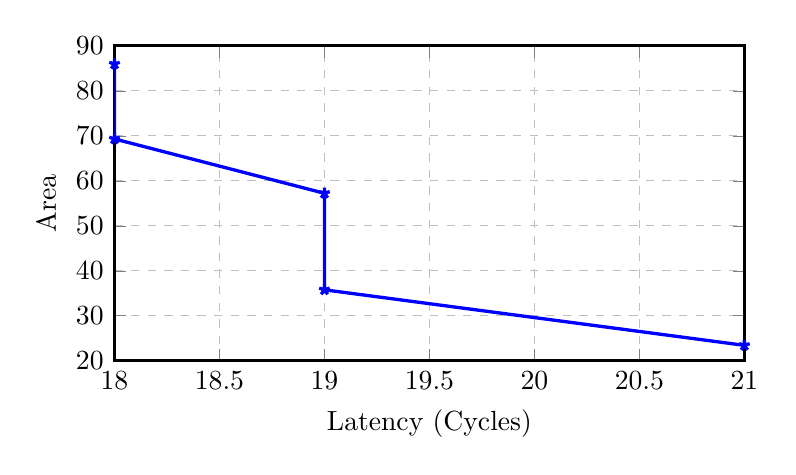
\begin{tikzpicture}
\begin{axis}[
scale only axis,
height=4cm,
width=8cm,
    xlabel={Latency (Cycles)},
    ylabel={Area},
    xmin=18, xmax=21,
    ymin=20, ymax=90,
    xtick={18,18.5,19,19.5,20,20.5,21},
    ytick={20,30,40,50,60,70,80,90},
    legend pos=north east,
    ymajorgrids=true,
    xmajorgrids=true,
    grid style=dashed,
    very thick
]
\addplot[
    color=blue,
    mark=star,
    %smooth
    ]
    coordinates {
    (18,85.95)(18,69.3)(19,57.225)(19,35.77)(21,23.429)
    };
\end{axis}
\end{tikzpicture}
\caption{Area Vs. Latency Curve for Butterfly Unit Implementation}
\label{plot_butterfly}
\end{figure}

From the graph, it can be seen that the latency value of 21 yields the minimum area. This value corresponds to the optimization, which limits the resources to one double precision adder subtractor unit and one double precision multiplier unit as given in table \ref{Table 4.1}. 

The results of design space exploration with the application of area optimization directives were compared against the results of the implementation with no optimization. The comparison is also given in table \ref{Table 4.1}.
\begin{table}[H]
\centering
\caption{Synthesis Results Comparison for Design Space Exploration for Butterfly Unit Execution for Resource Optimization for Zedboard ZC702}
\label{Table 4.1}
\begin{tabular}{||m{3cm}|m{2cm}|m{2cm}|m{2cm}|m{2cm}|m{2cm}||}
\hline
Metric & No Optimization & Resource Directive& Allocation Directive (3 Multipliers) & Allocation Directive (2 Multipliers) & Area Optimized  \\
\hline
\multicolumn{6}{||c||}{Timing Estimates}\\
\hline
Latency(Cycles) & 18 &18&19&19& 21\\
\hline
\multicolumn{6}{||c||}{Area Estimates}\\
\hline
Number of Multipliers & 4 & 4&3&2& 1\\
\hline
Number of Subtractors & 2 & 1&1&0&0\\
\hline
Number of Adders & 1 & 1&1&0&0\\
\hline
Number of Add-Sub Units & 1 & 0&0&1&1\\
\hline
DSP48E (\%age Utilization) & 25 & 22&17&11&6\\
\hline
LUT's (\%age Utilization) &13 & 8&8&4&4\\
\hline
Flip Flops (\%age Utilization) & 3 & 2&2&1&1\\
\hline
\end{tabular}

\end{table}

From table \ref{Table 4.1}, it can be seen that the resources are reduced by a significant factor i.e. the implementation is limited to use only one double precision multiplier and only one double precision adder-subtractor unit which is the minimum requirement for performing the calculations. However 3 cycles of latency are compromised. 

The resource utilization could be even lesser, if floating point data types are used e.g. the double precision multiplier uses 1149 LUT's to implement an adder unit, whereas the single precision floating point uses 390 LUT's to implement an adder unit.

\section {Analysis of 1024-Point FFT}\label {4.4}
The above implementation of butterfly unit is scaled up to compute a 1024 point FFT. The twiddle factors for computing the FFT are pre computed and supplied as array variables which are stored in BRAM to save the processing power at runtime. At a time two input samples are packed and sent to call the butterfly module which is already optimized by limiting the number of resources. Computation of N point FFT requires log\textsubscript{2}N stages, each computing N/2 butterfly operations.

The performance is further enhanced by exploring other pragmas available in Vivado HLS. e.g.
\begin{itemize}
\item
INLINE: This is used to replace function calls with function definitions. It is implemented by placing

\hspace{3cm}\# pragma HLS INLINE

at the beginning of the function body.
For computation of FFT the butterfly module is called several times, so it declared as INLINE using the above directive, to reduce the overhead of calling the functions.
\item
PIPELINE: This is used to use all resources concurrently in the algorithm. It is implemented by placing

\hspace{3cm}\# pragma HLS PIPELINE

\item
UNROLL: This is used to create multiple independent iterations of a loop simultaneously at the expense of resources. It is implemented by placing

\hspace{3cm}\# pragma HLS UNROLL \textit{unroll factor}

at the beginning of the loop body.
It should be noted the unroll factor must be provided otherwise the loop fails to unroll.
\end{itemize}

\noindent The design space exploration was performed for the FFT code with the application of different optimization pragmas as given in section \ref{4.4} and \ref{4.3.1}.

\noindent The performance analysis of the results of intermediate experiments of scaling the butterfly unit implementation to 1024 point FFT, which involves scaling the butterfly unit to first implement a 4-point FFT and then further scaling up to 16-point FFT and so on, is given as the area vs. latency curves as given in figure \ref {plot_4fft} to figure \ref{plot_128fft}.

The details of the design space exploration for the intermediate experiments is given in detail in tables \ref{4-point} to \ref{128-point}.


\begin{figure}[H]
\centering
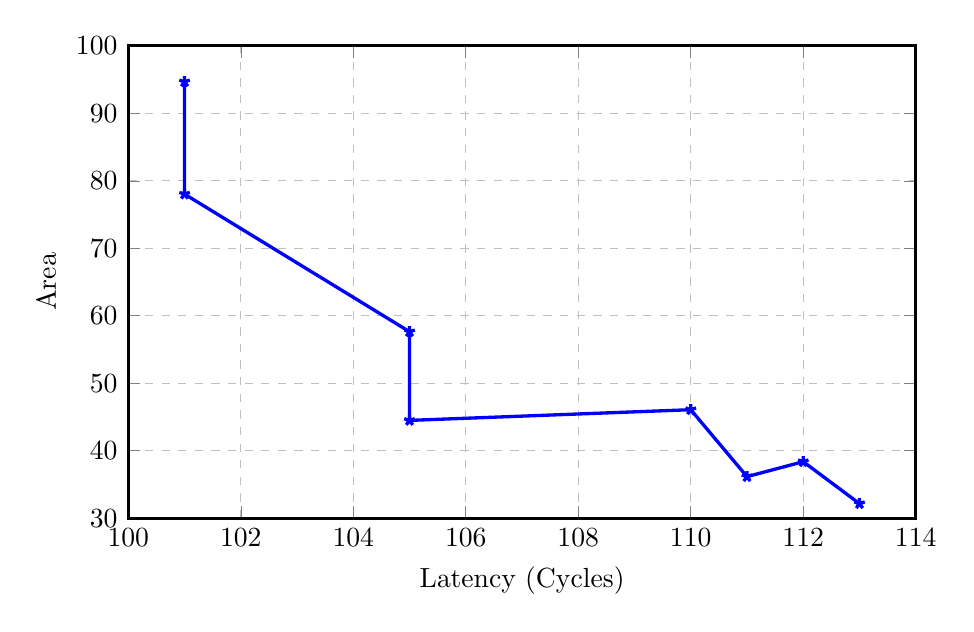
\begin{tikzpicture}
\begin{axis}[
scale only axis,
height=6cm,
width=10cm,
    xlabel={Latency (Cycles)},
    ylabel={Area},
    xmin=100, xmax=114,
    ymin=30, ymax=100,
    xtick={100,102,104,106,108,110,112,114},
    ytick={30,40,50,60,70,80,90,100},
    legend pos=north east,
    ymajorgrids=true,
    xmajorgrids=true,
    grid style=dashed,
    very thick
]
\addplot[
    color=blue,
    mark=star,
   % smooth
    ]
    coordinates {
    (101,94.675)(101,78.025)(105,57.6375)(105,44.495)(110,46.08)(111,36.165)(112,38.375)(113,32.166)
    };
\end{axis}
\end{tikzpicture}
\caption{Area Vs. Latency Curve for 4-Point FFT Implementation}
\label{plot_4fft}
\end{figure}
\begin{table}[H]
\centering
\caption{ Design Space Exploration Results for 4-Point FFT Computation for Zedboard ZC702}
\label{4-point}
\begin{tabular}{||m{1.5cm}|m{1.5cm}|m{1.5cm}|m{1.6cm}|m{1.6cm}|m{1.6cm}|m{1.4cm}|m{1.4cm}|m{1.4cm}||}
\hline
Metric & No Optimization & Resource & Allocation (3 Multipliers) & Allocation (2 Multipliers) & Allocation (1 multiplier) & Loop-1 Unroll (factor 2) & Loop 2-Unroll (factor 2) & Loop 1,2 Unroll (factor 2-2) \\
\hline
\multicolumn{9}{||c||}{Timing Estimates}\\
\hline
Latency (Cycles) & 101 & 101 & 105 & 105 & 113  & 112 & 111 & 110\\
\hline
\multicolumn{9}{||c||}{Area Estimates}\\
\hline
DSP48E  & 57 & 51 & 37 & 26 & 15 & 18 & 15 & 18\\
\hline
LUT's  &9042 & 6486 & 4953 & 4439 & 4120 &4890 & 5080 & 6740 \\
%\hline
%FF's & 4398 &3636 & 2822 & 2516 & 2137  &2287 & 2321 & 2647\\
\hline
\end{tabular}

\end{table}



\begin{figure}[H]
\centering
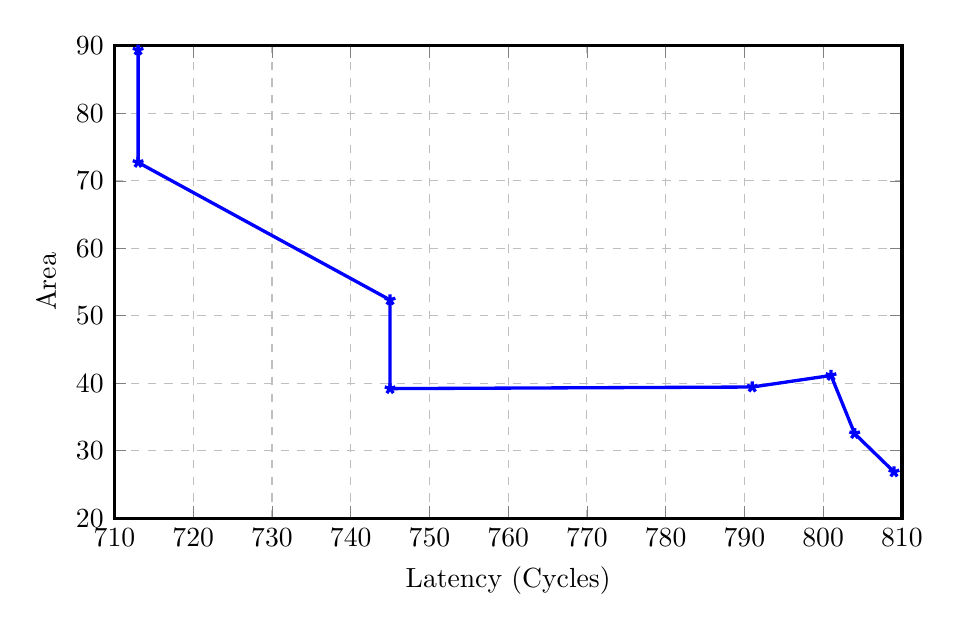
\begin{tikzpicture}
\begin{axis}[
scale only axis,
height=6cm,
width=10cm,
    xlabel={Latency (Cycles)},
    ylabel={Area},
    xmin=710, xmax=810,
    ymin=20, ymax=90,
    xtick={710,720,730,740,750,760,770,780,790,800,810},
    ytick={20,30,40,50,60,70,80,90},
    legend pos=north east,
    ymajorgrids=true,
    xmajorgrids=true,
    grid style=dashed,
    very thick
]
\addplot[
    color=blue,
    mark=star,
   % smooth
    ]
    coordinates {
    (713,89.37)(713,72.72)(745,52.345)(745,39.204)(791,39.441)(801,41.154)(804,32.54)(809,26.8625)
    };
\end{axis}
\end{tikzpicture}
\caption{Area Vs. Latency Curve for 16-Point FFT Implementation}
\label{plot_16fft}
\end{figure}
\begin{table}[H]
\centering
\caption{Design Space Exploration Results for 16-Point FFT Computation for Zedboard ZC702}
\label{16-point}
\begin{tabular}{||m{1.5cm}|m{1.5cm}|m{1.5cm}|m{1.6cm}|m{1.6cm}|m{1.6cm}|m{1.4cm}|m{1.4cm}|m{1.4cm}||}
\hline
Metric & No Optimization & Resource & Allocation (3 Multipliers) & Allocation (2 Multipliers) & Allocation (1 multiplier) & Loop-1 Unroll (factor 2) & Loop 1-Unroll (factor 4) & Loop 1,2 Unroll (factor 2-2) \\
\hline
\multicolumn{9}{||c||}{Timing Estimates}\\
\hline
Latency (Cycles) & 713 &713 &745 &745 & 809 & 804 & 801 & 791\\
\hline
\multicolumn{9}{||c||}{Area Estimates}\\
\hline
DSP48E  & 57 & 51 &37 & 26 &  15 & 18 & 22 & 18\\
\hline
LUT's  &7769 & 5213 & 3683 & 3169 & 2847 & 3490 & 4597 & 5146\\
%\hline
%FF's & 4199 & 3437 & 2612 & 2295 &  1916 & 2187 & 2622 & 2940\\
\hline
\end{tabular}

\end{table}

\begin{figure}[!h]
\centering
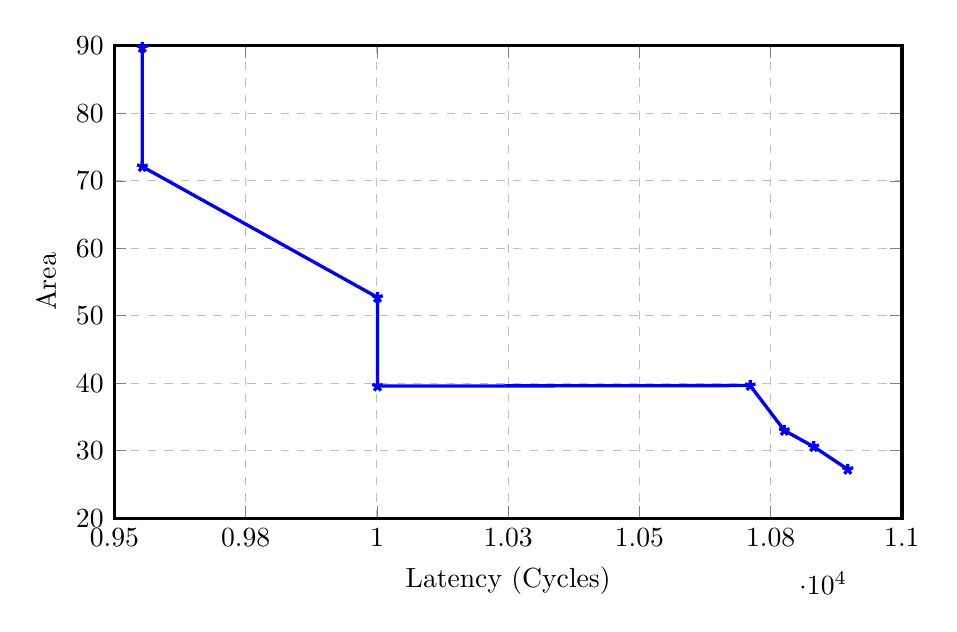
\begin{tikzpicture}
\begin{axis}[
scale only axis,
height=6cm,
width=10cm,
    xlabel={Latency (Cycles)},
    ylabel={Area},
    xmin=9500, xmax=11000,
    ymin=20, ymax=90,
    xtick={9500,9750,10000,10250,10500,10750,11000},
    ytick={20,30,40,50,60,70,80,90},
    legend pos=north east,
    ymajorgrids=true,
    xmajorgrids=true,
    grid style=dashed,
    very thick
]
\addplot[
    color=blue,
    mark=star,
   % smooth
    ]
    coordinates {
    (9553,89.745)(9553,72.098)(10001,52.720)(10001,39.579)(10711,39.658)(10776,33.004)(10832,30.595)(10897,27.2395)
    };
\end{axis}
\end{tikzpicture}
\caption{Area Vs. Latency Curve for 128-Point FFT Implementation}
\label{plot_128fft}
\end{figure}
\begin{table}[H]
\centering
\caption{Design Space Exploration Results for 128-Point FFT Computation for Zedboard ZC702}
\label{128-point}
\begin{tabular}{||m{1.5cm}|m{1.5cm}|m{1.5cm}|m{1.6cm}|m{1.6cm}|m{1.6cm}|m{1.4cm}|m{1.4cm}|m{1.4cm}||}
\hline
Metric & No Optimization & Resource & Allocation (3 Multipliers) & Allocation (2 Multipliers) & Allocation (1 multiplier) & Loop-1 Unroll (factor 2) & Loop 2-Unroll factor (2) & Loop 1,2 Unroll (factor 2-2) \\
\hline
\multicolumn{9}{||c||}{Timing Estimates}\\
\hline
Latency (Cycles) & 9553 & 9553 & 10001 &10001 & 10897 & 10776 &  10832 & 10711\\
\hline
\multicolumn{9}{||c||}{Area Estimates}\\
\hline
DSP48E  & 57 & 51 & 37 & 26 & 15 & 18 & 15 & 18\\
\hline
LUT's  &  7859 & 5303 & 3773 & 3259 & 2937 & 3603 & 3743 & 5198\\
%\hline
% FF's &  4145 & 3383 & 2558 & 2241 & 1862 & 2154 & 2183 & 2773\\

\hline
\end{tabular}

\end{table}





\noindent The utilization estimates by scaling the resource optimized butterfly for computing 1024 Point FFT are given in detail in table \ref{Table 4.3}.

\begin{table}[!h]
\centering
\caption{Synthesis Results Comparison for Resource Optimized 1024 Point FFT for Performance Optimization for Zedboard ZC702}
\label{Table 4.2}
\begin{tabular}{||m{4cm}|m{2.5cm}|m{2.5cm}|m{2.5cm}|m{2.5cm}||}
\hline
Metric & Area Optimized & INLINE & Pipeline & Unroll (Factor 8)\\
\hline
\multicolumn{5}{||c||}{Timing Estimates}\\
\hline
Clock (ns)&8.23 &8.23&8.23& 9.57\\
\hline
Latency(Cycles) &118805 & 118805 &119828 &126754\\
\hline
\multicolumn{5}{||c||}{Area Estimates}\\
\hline
DSP48E & 15& 15 &15 & 30 \\
\hline
LUT's & 3035 & 3035 &2909 &51644\\
\hline
Flip Flops & 1923 & 1923 & 2052 &16973\\
\hline	
\multicolumn{5}{||c||}{Profiling}\\
\hline
Time To compute FFT &1.19ms&1.19ms&1.2ms&1.27ms\\
\hline
\end{tabular}

\end{table}

The corresponding area vs. latency curve is given as:  \begin{figure}[!h]
\centering
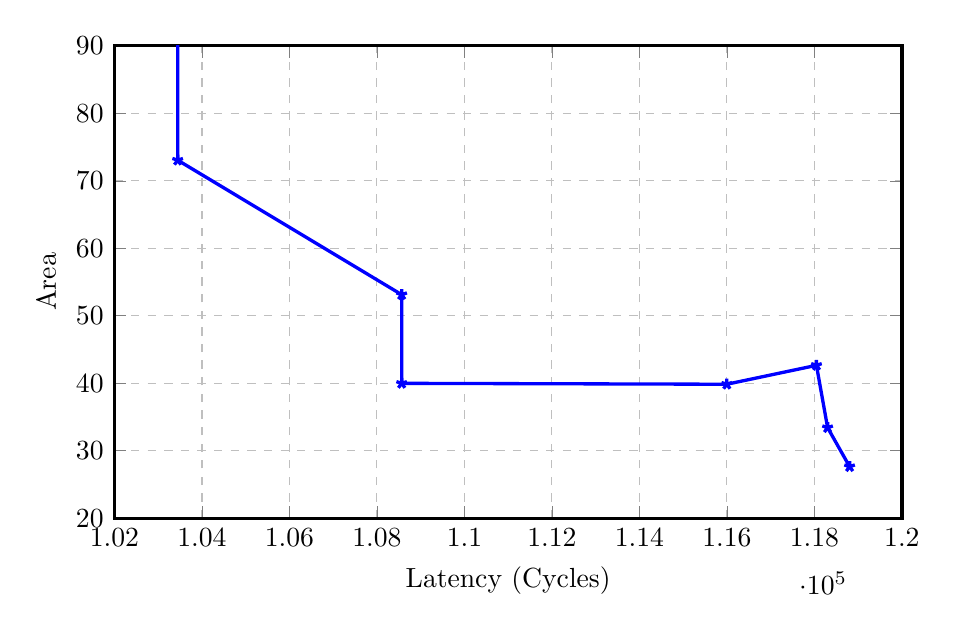
\begin{tikzpicture}
\begin{axis}[
scale only axis,
height=6cm,
width=10cm,
    xlabel={Latency (Cycles)},
    ylabel={Area},
    xmin=102000, xmax=120000,
    ymin=20, ymax=90,
    xtick={102000,104000,106000,108000,110000,112000,114000,116000,118000,120000},
    ytick={20,30,40,50,60,70,80,90},
    legend pos=north east,
    ymajorgrids=true,
    xmajorgrids=true,
    grid style=dashed,
    very thick
]
\addplot[
    color=blue,
    mark=star,
   % smooth
    ]
    coordinates {
    (103445,90.154)(103445,73.054)(108565,53.129)(108565,39.9875)(115998,39.854)(118047,42.654)(118302,33.425)(118805,27.646)
    };
\end{axis}
\end{tikzpicture}
\caption{Area Vs. Latency Curve for 1024-Point FFT Implementation}
\label{plot_1024fft}
\end{figure}

\noindent It should be noted that for computation of 1024 Point FFT:
\begin{itemize}
\item
The loops for execution of successive butterfly units are pipelined but it results in increase in the minimum clock period. 
\item
The loops used to compute FFT are unrolled by a factor of 8 which in turn ends up using almost 90 percent resources on Z702 zedboard as per the analysis in Vivado HLS. However only a few cycles of latency are saved. If more resources can be supplied, by changing hardware, more unroll options can be explored. 
\end{itemize}


All the above implementations use only one double precision multiplier and only one double precision adder-subtractor unit. Additions and subtractions are performed by the same adder-subtractor unit. 
From table \ref{Table 4.2}, if the time to compute 1024 Point FFT is computed it can be seen that it takes minimum as 1.19ms sec by the area optimized FFT. The unroll by a factor of 8 consumes almost 97 percent of LUT's for Zedboard(ZC702). To explore further parallelism we might need to use other hardware which supplies more number of resources. 

%\section{Performance Analysis by changing the Underlying Hardware}
%The given area optimization's are applied to Virtex VC709 board for the same algorithm and the results were compared in terms of resource consumption, latency and time taken to compute the 1024 point FFT. The comparison is as described in table \ref{Table 4.3}.

%The choice of platform depends on a lot of factors e.g. cost, area, performance requirements, e.g. If a latency optimized designed is required, parallelism should be exploited at the expense of resources, as the total number of resources are more. 

For efficient implementation of FHEW on hardware, the area optimized FFT algorithm can be used as a packaged core and can be used to provide executions of several FFT's running in parallel to increase the speed of algorithm. 

%\begin{table}[!h]
\centering
\begin{tabular}{||m{5.5cm}|m{4cm}|m{4cm}||}
\hline
Metric & Virtex (VC709) & Zedboard (ZC702)  \\
\hline
\multicolumn{3}{||c||}{Timing Estimates}\\
\hline
Estimated Clock (ns) & 9.83 & 8.23\\
\hline
Latency (Cycles) &98325&118805\\
\hline
\multicolumn{3}{||c||}{Area Estimates}\\\cline{1-3}

DSP48E & 15 & 15\\
\hline
LUT's &2238 & 3035\\
\hline
Flip Flops  &1862 & 1923\\
\hline
\multicolumn{3}{||c||}{Profiling}\\
\hline
Time To compute FFT &98.3us& 1.19ms\\
\hline
\end{tabular}
\caption{Performance Comparison of Double Precision Area optimized FFT on VC709 and ZC702 board}
\label{Table 4.3}
\end{table}

In the next chapter another computationally intensive algorithm, deep neural network is explored for modification in arithmetic from floating point to fixed point.





\chapter{Arithmetic of a Deep Neural Network}\label{Chapter5}
\section {Digit Recognition Problem}
The MNIST data set is a set of images ($28\times 28$ size) of handwritten digits from 0-9, of which about 10000 are for testing the network and 60000 are for training the network.
Lenet 5 is a model designed for classification and recognition of images.
Convolutional layer and max pool layer are two important features of the lenet family of models.
The implementation supported in [\ref{papaa}] is a working opencl implementation of lenet 5 model to classify the digits in MNIST data set. Also it has many labs to analyze the performance for CPU and GPU.
\subsection{Detailed Explanation of the Implementation}
The current library uses OPENCV which is a library written in C++ developed for computer vision applications. The entire implementation uses 32 bit single precision float data type to store the convolution weights, filters and biases for various layers. The lenet model in the library is a trained model which is trained using Caffe. The weights are stored in a file \textit{"lenet5\_model.cpp"}.
The application supports 8 layers as demonstrated in figure \ref{fig:Lenet Application}. %figure
%image: 

\begin{figure}[h]
\centering
\includegraphics[scale=0.8]{figures/lenet5.PNG}
\caption{Lenet Model for MNIST Data Set Classification}
\label{fig:Lenet Application}
\end{figure}
\subsubsection{Convolution Layer 1}\label{Convolution layer 1}
In this layer a set of filters are slided spatially on the image to perform a 2 dimensional convolution operation. The layer takes 1 image of $[28\times 28]$ size as input and yields an output vector of size $[24\times 24 \times 20]$ considering that 20 filters are applied. The filter matrices are of dimension $[5\times 5]$ and contain single precision float values. 

\noindent The $[5\times 5]$ filters may have different values based on the features e.g. features representing small objects or regions in  an image e.g. edges , color, lines etc. The convolution layer 1 produces 20 filters where each filter is a $[24\times 24]$ map. The maps are stacked one over the other to produce the output.
\subsubsection{Max Pool Layer 1}\label{Max Pool layer 1}
Max pool layer is generally placed between two convolution layers. It performs a down sampling operation along the spatial dimensions which helps in reduction of parameters and computations. 

It takes the output maps from convolution layer 1 as input and applies a max operation on each $[2\times 2]$ slice of input i.e. (maximum of 4 values) is taken with a sliding step of 2 resulting in reduction of image size per image as $[12\times 12]$, however the number of maps remain the same.

\noindent It takes input of size $w\times h\times d$ $[24\times 24\times 20]$

\noindent Uses two parameters window size (z) and step size (s)  (2,2)

\noindent Produces an output of volume: $w'= (w-z)/s+1$, $h'= (h-z)/s+1$ and $d'=d$
\subsubsection{Convolution Layer 2}\label{Convolution layer 2}
It performs a 2D convolution operation as referenced in \ref{Convolution layer 1} on output volume from max pool layer 1. It takes a volume of size $[12\times 12\times 20]$ as input and generates an output volume of size $[8\times 8\times 50]$, specifying 50 filters on the given input. The filter size used is same as in \ref{Convolution layer 1} i.e. $[5\times 5]$.
\subsubsection{Max Pool Layer 2}\label{Max Pool layer 2}
From the output of convolution layer 2, again a down sampling operation is performed and an output volume is generated which has a dimension of $[4\times 4\times 50]$.
\subsubsection{Inner Product Layer 1}\label{Inner Product Layer 1}
It is a fully connected layer wherein the neurons have full connections to all the  activation maps of the previous layer. The fully connected layer is converted to a convolution layer i.e. the input volume of size $[4\times 4\times 50]$ is converted to an input of $[1\times 800]$ considering the layer has 800 bias. The output of inner product layer is $[1\times 500]$ volume, which  involves 500 1D convolution of two $[1\times 800]$ matrices.
\subsubsection{Relu Layer}\label{Relu Layer}
Relu layer applies an element wise activation function, i.e. if the output is less that 0, it will set it to 0. The output dimensions are same as input.
\subsubsection{Inner Product Layer 2}\label{Inner Product Layer 2}
The output of relu layer is processed with another fully connected layer with 500 filters, which yields an output $[1\times 10]$.
It produces the class scores based on the digits 0-9 resulting in an output of size $[1\times 1\times 10]$.
\subsubsection{Soft Max Layer}\label{Soft Max Layer}
It produces output probabilities based on the class scores.

\vspace{0.25cm}
\noindent The most computationally intense part in the above implementation is convolution operation.

\section{Fixed Point Mathematics Implementation:}
The 2 dimensional convolution operation performs a multiplication operation and then the result of this multiplication is added to the output variable for the $[5\times 5]$ overlap region of the input image and filter.
Functions are written to implement the above three operations in fixed point.

\vspace{0.25cm}
\subsection{Float to Fixed Format Conversion:}

\vspace{0.25cm}
\noindent It is used to convert the initial input value and filter value in the fixed point format by using the methodology described in section \ref{2.5.3}. It uses the roundf() function from the C++ maths library, which computes the nearest integer value to the floating point argument.

\lstset { %
	language=C,
	backgroundcolor=\color{lightgray}, % set backgroundcolor
	%basicstyle=\footnotesize,% basic font setting
	basicstyle=\ttfamily\scriptsize,
	%\basicstyle=\ttfamily\scriptsize,
	keywordstyle=\color{blue}\ttfamily,
	stringstyle=\color{red}\ttfamily,
	commentstyle=\color{darkgray}\ttfamily,
	breaklines=true	
}
\lstset{framesep=-10pt, xleftmargin=-10pt}
\begin{lstlisting} [caption={Sample Code to Convert from Float to Fixed}
,label={listing:2}]
int convert(float num1)
{
     int c;
     float b;
     
     //Scale floating point variable num1 up by a factor 2^frac_len
     b=num1*(2^frac_len);
     
     //use the Round function in the math library of C++ 
     //to round the variable to nearest integer.
     c=roundf(b);
     
     return(c);
}
\end{lstlisting}



\vspace{0.25cm}
\subsection{Fixed Point Addition:}

\vspace{0.25cm}
\noindent In the 2 dimensional convolution operation, the input and filter are converted in same Q32.\textit{frac\_len} format. The addition is performed for two numbers in same Q format as described in section \ref{2.5.3}.

\lstset { %
	language=C,
	backgroundcolor=\color{lightgray}, % set backgroundcolor
	%basicstyle=\footnotesize,% basic font setting
	basicstyle=\ttfamily\scriptsize,
	%\basicstyle=\ttfamily\scriptsize,
	keywordstyle=\color{blue}\ttfamily,
	stringstyle=\color{red}\ttfamily,
	commentstyle=\color{darkgray}\ttfamily,
	breaklines=true	
}
\lstset{framesep=-10pt, xleftmargin=-10pt}
\begin{lstlisting}[caption={Sample Code for Fixed Addition},label={listing:3}]
float addition (float num1,float num2)
{
     int n1,n2;
     float temp_result;
  
     //Convert num1 and num2 to fixed point using the function convert
     //as given in section 4.2.3
     n1=convert(num1);
     n2=convert(num2);
  
     //Return the result of fixed point addition
     temp_result=n1+n2;
  
     return temp_result;
}
\end{lstlisting}



\noindent In the above sample, the numbers are converted to fixed point and the result of addition is returned in fixed point format. The result can be converted back to float by scaling with a factor of $2^{-frac\_len}$ or can be used as it is in case of successive fixed point additions.

\vspace{0.25cm}
\subsection{Fixed Point Multiplication:}

\vspace{0.25cm}
\noindent The 2 dimensional convolution operation is implemented to perform a fixed point multiplication on two numbers in the same Q format as described in Listing \ref{listing:4}.
\noindent 

\lstset { %
	language=C,
	backgroundcolor=\color{lightgray}, % set backgroundcolor
	%basicstyle=\footnotesize,% basic font setting
	basicstyle=\ttfamily\scriptsize,
	%\basicstyle=\ttfamily\scriptsize,
	keywordstyle=\color{blue}\ttfamily,
	stringstyle=\color{red}\ttfamily,
	commentstyle=\color{darkgray}\ttfamily,
	breaklines=true	
}
\lstset{framesep=-10pt, xleftmargin=-10pt}
\begin{lstlisting}[caption={Sample Code for Fixed Multiplication},label={listing:4}]
float multiply(float num1,float num2)
{
     int temp;
     int n1,n2;
     float temp_result; 
     
     //Convert num1 and num2 to fixed point using the function convert
     //as given in section 4.2.3
     n1=convert(num1); 
     n2=convert(num2);
    
     //compute Fixed Point Multiplication
      temp=n1*n2;
      
     //adjust the result of fixed point multiplication
     //by scaling down with 2^frac_len
      temp_result=temp/(2^frac_len);
      
      return temp_result;
}
\end{lstlisting}


\noindent The above sample takes two floating point numbers as input and returns the result of multiplication in fixed point format. The extra scaling by a factor of $2^{-frac\_len}$ specific to the multiplication operation as described in section \ref{2.5.3} is already performed. To convert the result back to floating point representation, the result returned from the function should be scaled by a factor of $2^{-frac\_len}$.
\section{Introduction to Libfi}
Libfi is a free open source template based header based binary fixed point library for C++, intended to be used for hardware.
\subsection{Main Features}
The library offers various features like, customizable rounding and overflow handling modes etc.
\subsubsection{Libfi: Fixed Data type}
The fixed point data type under the namespace \textit{Fi} takes 5 parameters.
\begin{enumerate}
\item
\textbf{W:} It represents the total word length in bits, including the sign bit. W must be less than or equal to 32, however it does not necessarily have to be a power of two.
\item
\textbf{F:} It represents the number of fractional bits. F Must be less than or equal to W.
\item
\textbf{S:} It represents the signedness of the resulting type. Values for S are:

\noindent Signed denoted by (Fi::SIGNED) and

\noindent Unsigned denoted by (Fi::UNSIGNED).

\item
\textbf{OF:} It specifies the overflow handling mode for the fixed point number. It defaults to wrap-around. The other overflow handling modes are described in \ref{Overflow Section}. 
\item
\textbf{R:} It specifies the rounding mode. It defaults to rounding towards zero. The other rounding modes are described in \ref{Rounding Modes Section}.
\end{enumerate}
\vspace{0.5cm}
\textbf{Example Representations}

Fi::Fixed\textless8, 4, Fi::SIGNED, Fi::Wrap\textgreater a("3.14");

defines a signed fixed point variable having word length 8, fractional length 4, with the overflow handler \textit{wrap} representing value 3.14.

\vspace{0.5cm}
Fi::Fixed\textless8, 4, Fi::UNSIGNED, Fi::Saturate\textgreater a("3.14");

defines an unsigned fixed point variable having word length 8 and fractional length 4, with the overflow handler \textit{saturate} representing value 3.14.

\vspace{0.25cm}
\noindent Multiple constructors of the class \textit{Fixed} allow creation of fixed objects from floating point numbers, strings representing fixed point number or from other fixed point objects.
It also allows creation of a fixed object from a raw binary value representing a fixed point number.
Various logical operations are implemented e.g. Bitwise AND, OR, Comparison, Shifting operations etc.
\subsubsection{Libfi: Rounding Modes}\label{Rounding Modes Section}
The library offers various fixed point rounding modes each of which is implemented with a separate round function in structure variables defining the modes.
\begin{enumerate}
\item
\textbf{NearOdd:} A value is rounded towards the nearest value, except for ties which are settled towards the nearest odd value.

\noindent The input is the fixed point number to be rounded and the rounded value alongwith a -1(+1) indicating that positive(negative) numbers can decrease(increase) in value as a result of rounding or 0 if the input is zero is returned.
\item
\textbf{NearEven:} A value is rounded towards the nearest value except for ties which are settled towards the nearest even value.

\noindent The input is fixed point number to be rounded and the rounded value alongwith a -1(+1) indicating that positive(negative) numbers can decrease(increase) in value as a result of rounding, or 0 if the input is zero is returned.
\item
\textbf{Floor:} A value is rounded towards negative infinity which  is also known as floor or negative. It always assumes that bits representing the fractional length will be rounded away.

\noindent The input is fixed-point number to be rounded and it returns the rounded value and -1 indicating that numbers can increase in value as a result of rounding, or 0 if the input is 0.
\item
\textbf{Fix:} A value is rounded towards zero, which is also known as fix or away from infinity. As rounding to floor, it also assumes that fractional length bits will be rounded away.

\noindent The input here in is the Fixed-point number to be rounded. It returns The rounded value and -1 (+1) indicating that positive (negative) numbers can decrease (increase) in value as a result of rounding, or 0 if the input is zero.	
\item
\textbf{Classic:}A value is rounded(up or down) towards nearest value. Ties are rounded away from zero.

\noindent It takes the fixed point number to be rounded as input and returns the rounded value and -1(+1) indicating that positive(negative) numbers can decrease (increase) in value.

\item
\textbf{Ceil:} A value is rounded towards positive infinity. It assumes that bits representing the fractional length will be rounded away.

\noindent The input is fixed point number to be rounded and it returns the rounded value and 1 indicating that numbers can increase in value as a result of rounding,or 0 if the input is 0.
\end{enumerate}

\subsubsection{Libfi: Overflow}\label{Overflow Section}
The library offers various modes to handle overflows as described below:
\begin{enumerate}
\item
\textbf{Wrap Around:} A wrap around(modulus) overflow handler. 

\noindent If overflow occurs, the assigned value is the original value modulo $2^{(W+1)}$.
The input is the integer representing a fixed-point number and the return value is the number after wrapping is applied.
\item
\textbf{Saturate:} A saturating overflow handler.

\noindent If overflow occurs, the assigned value is set to nearest representable value. The input is the integer representing a fixed-point number and the return value is the number after saturation is applied.
\item
\textbf{Throw:} Throws an exception when overflow occurs.

\noindent If positive overflow occurs, Fi::PositiveOverflow is thrown.

\noindent If negative overflow occurs, Fi::NegativeOverflow is thrown.

\noindent The input is the integer representing a fixed-point number and the number provided in throws std::overflow\_error is returned.
\item
\textbf{Undefined:} It is used if undefined behavior in the event of an overflow can be accepted. Currently, the only advantage of using this over other overflow handler is a minor speed improvement as it is optimized for speed, although the actual behavior depends on the compiler and underlying system.

\noindent It takes the integer representing a fixed-point number as input and returns the number or a warning that the programmer is willing to accept undefined behavior in the event of an overflow.
\end{enumerate}

\section{Integration of Libfi with Existing Implementation of MNIST Data Set Classification}
Before downloading the library, Opencv needs to be setup in Linux and the path should be setup using LD\_LIBRARY\_PATH.
The library can be downloaded from the git repository as mentioned in [\ref{lib}]. The header files referencing various functions of \textit{Libfi} as specified below:

\noindent "fi/Fixed.hpp"

\noindent "fi/overflow/Wrap.hpp"

\noindent need to be added in the main file of \textit{Lenet5} application code file.
\begin{itemize}
\item
\textbf{Libfi: Conversion from Float to Fixed}

\noindent Considering a float point variable "X", a corresponding fixed point variable with specified word length (WL) and fractional length (FL) can be defined as:

\hspace{3cm}Fi::Fixed\textless WL, FL, Fi::SIGNED\textgreater a(X);

\noindent Here "a" represents the converted value of a floating point variable X with word length (WL) out of which FL represents the number of bits for fractional part.
\item
\textbf{Libfi: Conversion from Fixed to Float}

\noindent Considering a fixed point variable "a", with word length (WL) and fractional length (FL), the corresponding floating point converted variable "X" can be defined as:

\hspace{3cm}X = a.toFloat();

\noindent Here "X" represents the converted value of a fixed point variable "a" with word length (WL) out of which FL represents the number of bits for fractional part.
\item
\textbf{Libfi: Fixed Point Multiplication Example}

\noindent Considering two fixed point variables "a" and "b" defined with a word length (WL) and fractional length (FL), a fixed point multiplication can be performed as:

\lstset { %
	language=C,
	backgroundcolor=\color{lightgray}, % set backgroundcolor
	%basicstyle=\footnotesize,% basic font setting
	basicstyle=\ttfamily\scriptsize,
	%\basicstyle=\ttfamily\scriptsize,
	keywordstyle=\color{blue}\ttfamily,
	stringstyle=\color{red}\ttfamily,
	commentstyle=\color{darkgray}\ttfamily,
	breaklines=true	
}
\lstset{framesep=-10pt, xleftmargin=-10pt}
\begin{lstlisting}[caption={Libfi:Fixed Point Multiplication Example Code Snippet},label={listing:5}]
//include Fixed Point Library files.
#include "fi/Fixed.hpp"
#include "fi/overflow/Wrap.hpp"
#include <iostream>

#define WL 8
#define FL 4

int main(int argc, char* argv[]) 
{
     //Define two fixed point variables a and b
     Fi::Fixed<WL, FL, Fi::SIGNED> a("3.14");
     Fi::Fixed<WL, FL, Fi::SIGNED> b("1.14");
  
     //Display the result of Fixed Point multiplication.
     std::cout << a*b << std::endl;
  
     return 0;
}
\end{lstlisting}




\end{itemize}
\noindent The code snippet in listing \ref{listing:5} is written referring to the examples given in [\ref{lib}]. In the above example a fixed point multiplication operation is performed on two fixed Point variables: "a" having the value 3.14 and "b" having the value 1.14, stored in fixed point format with a word length 8 and fractional length 4 and the result is displayed on screen. The corresponding result obtained is 3.5. By performing the multiplication in floating point the corresponding result is 3.5796. The difference in values is because of the rounding off errors introduced by using fixed point format. 

\vspace{0.25cm}
The convolution layers 1 and 2 of the application use a function \textit{CustomFilter2D} which performs a two dimensional convolution in floating point data types, on the feature maps with a 5 * 5 kernel as described in section \ref{Convolution layer 1} and \ref{Convolution layer 2}. In the 2D convolution operation, multiply accumulate operation is performed on two 5*5 matrices. The overlapping numbers of two matrices are multiplied and then the result of the multiplication is accumulated to generate a value.

\vspace{0.25cm}
The two dimensional convolution function is modified such that, the inputs are first converted in fixed points, and the fixed point multiplication is computed and the result is converted back to float and accumulated in the floating variable. The sample code snippet given in \ref{listing:61} describes the operation.


\lstset { %
	language=C,
	backgroundcolor=\color{lightgray}, % set backgroundcolor
	%basicstyle=\footnotesize,% basic font setting
	basicstyle=\ttfamily\scriptsize,
	%\basicstyle=\ttfamily\scriptsize,
	keywordstyle=\color{blue}\ttfamily,
	stringstyle=\color{red}\ttfamily,
	commentstyle=\color{darkgray}\ttfamily,
	breaklines=true	
}
\lstset{framesep=-10pt, xleftmargin=-10pt}
\begin{lstlisting}[caption={Two Dimensional Convolution Operation Code Snippet},label={listing:61}]

out.at<float>(r,c) = 0;

for(int i = 0; i < ker.rows; i++) {

  for(int j = 0; j < ker.cols; j++) {   
    
    //Define a fixed point variable "a"
    //to store the fixed point value of kernel
    Fi::Fixed<word_length, frac_length, Fi::SIGNED> a(ker.at<float>(i, j));
    
    //Define a fixed point variable "b" 
    //to store the fixed point value of Input
    Fi::Fixed<word_length, frac_length, Fi::SIGNED> b(input.at<float>(r+i, c+j));
    
    //Define a fixed point variable "temp1" 
    //to store the result of fixed point multiplication
    Fi::Fixed<word_length, frac_length, Fi::SIGNED> temp1(a*b);
    
    //the result is converted back to float and added to the output.
	out.at<float>(r,c) += temp1.toFloat();
	
	}
}
\end{lstlisting}

\vspace{0.25cm}
In the code, given in listing \ref{listing:61}
\begin{itemize}
\item
\textit{word\_length} and \textit{frac\_length} are two macros defined to represent the number of bits to represent fixed point word and the number of bits used to represent the fractional part.
\item
\textit{ker} is a 5*5 matrix, which represents the weights.
\item
For each 5*5 matrix multiplication, fixed point variable \textit{"a"} stores the fixed point converted value corresponding to a floating point value of \textit{ker} at a point.
\item
Similarly fixed point variable \textit{"b"} stores the fixed point converted value corresponding to a floating point value of \textit{input} at a point.
\item
The variable \textit{"temp1"} stores the result of the fixed point multiplication of \textit{a} and \textit{b}.
\item 
The result stored in \textit{"temp1"} is converted back to float and accumulated in the floating value at a point represented by \textit{out}.
\item 
The entire multiplication is performed in signed arithmetic with default rounding and overflow handling modes.
\end{itemize}
\noindent The \textit{"Fi"} folder under the \textit{Libfi} library is copied in the folder containing the C++ references for the implementation of MNIST data set classification. Makefile is updated to include the path of \textit{Libfi}, under the \textit{CPPFLAGS} link to avoid the include errors. Another way is to update the include path in all source files of \textit{Libfi} library.


\lstset { %
	language=C,
	backgroundcolor=\color{lightgray}, % set backgroundcolor
	%basicstyle=\footnotesize,% basic font setting
	basicstyle=\ttfamily\scriptsize,
	%\basicstyle=\ttfamily\scriptsize,
	keywordstyle=\color{blue}\ttfamily,
	stringstyle=\color{red}\ttfamily,
	commentstyle=\color{darkgray}\ttfamily,
	breaklines=true	
}
\lstset{framesep=-10pt, xleftmargin=-10pt}
\begin{lstlisting}[caption={Changes to Makefile},label={listing:6}]
include ./sources.mk

exec=lenet_app

CC=g++

CPPFLAGS=CPPFLAGS= -g $(shell pkg-config --cflags opencv)\
          -I/usr/local/include/opencv2\
           -I./fi -I ./
           
LIBS= $(shell pkg-config --libs opencv) -lpapi 
\end{lstlisting}



\noindent The application can be build by running the \textit{"make all"} command in the command line, with \textit{cpp-ref} folder as the working directory.

\vspace{0.25cm}
\noindent To check the result of a single image classification, the following command should be executed:

\vspace{0.25cm}
./lenet\_app -m sample -i ../imgs/mnist\_test\_img\_0.pgm

\vspace{0.25cm}
\noindent Here \textit{mnist\_test\_img\_0.pgm} is the image name. The results can be tested for other user specified images also.

\vspace{0.25cm}
\noindent To test the library for whole dataset of 10000 images, the test images folder in the \textit{imgs} folder of the library should be expanded followed by the execution of the following command :

\vspace{0.25cm}
./lenet\_app -m test -f ../imgs/mnist\_test\_img\_list.csv -d ../imgs/mnist-testset

\vspace{0.25cm}
\noindent \textbf{Sample Output:} The sample output for the execution of entire test set is as shown in figure \ref{fig:output_mnist}.

\begin{figure}[!h]
\centering
\includegraphics[scale=0.65]{figures/sample_output.png}
\caption{Sample Output for Test set of 10000 Images}
\label{fig:output_mnist}
\end{figure}
\noindent The existing implementation was simulated for combinations of word length and fractional length, keeping the word length as 32. The tests are run for MNIST test set comprising of 10000 images and the accuracy is computed in terms of number of images which are correctly classified.

\noindent The effect on accuracy of classification algorithm by varying the fixed point fractional length for word length of 32 and 16 are shown in table \ref{Results Fixed1} and \ref{Results Fixed2}.

\begin{table}[h]
\centering
\caption{Effect on Accuracy by varying the Fixed Point Fractional Length (Word Length 32).}
\label{Results Fixed1}
\begin{tabular}{||m{3cm}|m{1.5cm}|m{1.5cm}|m{1.5cm}|m{1.5cm}|m{1.5cm}|m{1.5cm}||}
\hline
\multirow{2}{*}{Metric} & \multirow{2}{*}{\parbox{1.5cm}{Floating Point Datatype}} & \multicolumn{5}{|c||}{ Fixed Point Fractional Length (Word Length 32)} \\[1.5ex]\cline{3-7}
& & 16bits&12 bits &8bits&4bits&2bits \\[1.5ex]
\hline
\hline
Number of images wrongly classified   & 95 &95 &95 &96 &567 &8865\\
\hline
Number of images correctly classified &9905&9905&9905&9904&9433&1135\\
\hline
Accuracy (\% of images correctly classified)&99.05\%&99.05\%&99.05\%&99.04\%&94.33\%&11.35\%\\
\hline
\end{tabular}

\end{table}

\begin{table}[!h]
\centering
\caption{Effect on Accuracy by varying the Fixed Point Fractional Length (Word Length 16).}
\label{Results Fixed2}
\begin{tabular}{||m{4cm}|m{2cm}|m{1.5cm}|m{1.5cm}|m{1.5cm}|m{1.5cm}||}
\hline
\multirow{2}{*}{Metric} &  \multicolumn{5}{|c||}{ Fixed Point Fractional Length (Word Length 16)} \\\cline{2-6}
& 16bits&12 bits &8bits&4bits&2bits \\
\hline
\hline
Exception& Positive Overflow &\multicolumn{4}{|c||}{-}\\
\hline
Number of images wrongly classified    &- &95 &96 &567 &8865\\
\hline
Number of images correctly classified  &- &9905&9904&9433&1135\\
\hline
Accuracy (\% of images correctly classified)&- &99.05\%&99.04\%&94.33\%&11.35\%\\
\hline
\end{tabular}

\end{table}
\noindent The effect of changing the fixed point bit-width on the accuracy can be seen in a more detailed manner from \ref{fig:graph}.
 \begin{figure}[!h]
\centering
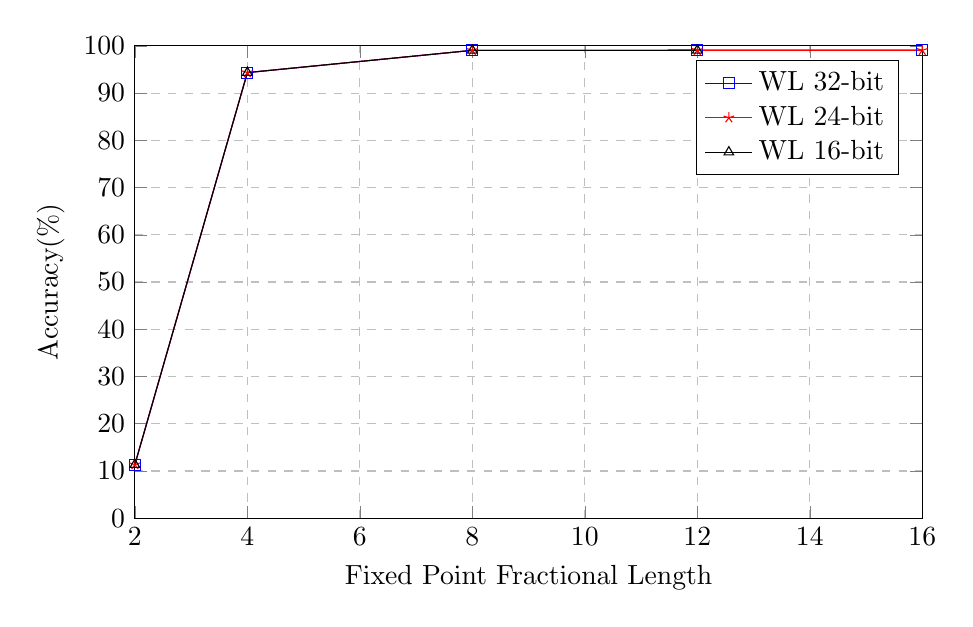
\begin{tikzpicture}
\begin{axis}[
scale only axis,
height=6cm,
width=10cm,
    xlabel={Fixed Point Fractional Length},
    ylabel={Accuracy(\%)},
    xmin=2, xmax=16,
    ymin=0, ymax=100,
    xtick={2,4,6,8,10,12,14,16},
    ytick={0,10,20,30,40,50,60,70,80,90,100},
    legend pos=north east,
    ymajorgrids=true,
    xmajorgrids=true,
    grid style=dashed,
]
\addplot[
    color=blue,
    mark=square,
    ]
    coordinates {
    (2,11.35)(4,94.33)(8,99.04)(12,99.05)(16,99.05)
    };
    \addlegendentry{WL 32-bit}
 \addplot[
    color=red,
    mark=star,
    ]
    coordinates {
    (2,11.35)(4,94.33)(8,99.04)(12,99.05)(16,99.05)
    };
   \addlegendentry{WL 24-bit}
  \addplot[
    color=black,
    mark=triangle,
    ]
    coordinates {
    (2,11.35)(4,94.33)(8,99.04)(12,99.05)
    };
   \addlegendentry{WL 16-bit}
\end{axis}
\end{tikzpicture}
\caption{Effect of varying the Fractional Length on Accuracy}
\label{fig:graph}
\end{figure}
\vspace{0.25cm}
\noindent It should be noted that for the given Lenet model, the accuracy increases with the increase in the number of fractional bits by keeping the fixed point word length constant. Because as the number of bits to store the fractional bits are increased, the system becomes more efficient to precisely store the values after the decimal point which in the course of algorithm after successive multiplications and additions may effect the reliability if not handled properly.

\vspace{0.25cm}
\noindent In this model, changing the word length also doesn't affect the readings, because the values are normalized and lie between 0 to 1. The result throws a positive overflow exception for Q16.16 combination of the fixed point which implies zero bits are supplied to store the integer part. So it cannot be simulated for Q16.16 format.

\vspace{0.25cm}
\noindent From the above results, it is verified that the accuracy for fixed point formats Q24.16 and Q32.16 is same as that of float.

\section{Introduction to HLS Arbitrary Precision Fixed Point Library}
The fixed point functions for hardware can be implemented using the inbuilt class in Vivado HLS for arbitrary precision fixed point types in C++ which can be accessed by including the header file:

\hspace{3cm}\#include\textless ap\_fixed.h\textgreater

\noindent There are separate classes for signed and unsigned numbers e.g.

\hspace{3cm}ap\_fixed for Signed and 

\hspace{3cm}ap\_ufixed for Unsigned
\begin{itemize}
\item
\textbf{Fixed Point Representation:}
A fixed point number in the above class can be represented as:

ap\_[u]fixed\textless int W, int I, ap\_q\_mode Q, ap\_o\_mode O, ap\_sat\_bits N\textgreater;

In the above representation:
\begin{itemize}
\item
\textbf{W :} W represents the word length
\item
\textbf{I :} I represents the number of bits to represent integer part. This implies the number of bits used to represent the fractional part is W-I.
\item
\textbf{ap\_q\_mode Q :} It represents the quantization mode. There are multiple options supported by Vivado HLS for quantization modes as mentioned in table \ref{rounding}.
\begin{table}[!h]
\centering
\begin{tabular}{m{4cm} m{6cm}}
AP\_RND & Rounding to plus infinity\\
AP\_RND\_ZERO & Rounding to zero\\
AP\_RND\_MIN\_INF & Rounding to minus infinity\\
AP\_RND\_INF & Rounding to infinity\\
AP\_RND\_CONV & Convergent rounding\\
AP\_TRN (default) & Truncation\\
AP\_TRN\_ZERO & Truncation to zero
\end{tabular}
\caption{Vivado HLS Fixed Point Rounding Modes}
\label{rounding}
\end{table}
\item
\textbf{ ap\_o\_mode O :} It represents the overflow mode. Various overflow modes supported by Vivado HLS are mentioned in table \ref{overflow}.

\begin{table}[!h]
\centering
\begin{tabular}{m{4cm} m{6cm}}
AP\_SAT & Saturation\\
AP\_SAT\_ZERO& Saturation to zero\\
AP\_SAT\_SYM & Symmetrical saturation\\
AP\_WRAP & Wrap-around\\
AP\_WRAP\_SM&Sign magnitude wrap-around\\
\end{tabular}
\caption{Vivado HLS Fixed Point Overflow Modes}
\label{overflow}
\end{table}
\item
\textbf{ap\_sat\_bits N:} It represents the number of saturation bits. The saturation is executed based on the value of N.
\end{itemize}

\item
\textbf{Conversion from Fixed to other Datatypes:}
There are member functions to convert the fixed point variable to other datatypes e.g. float, double etc. 

\hspace{3cm} double ap\_[u]fixed::to\_double()

The above function can be used to convert a fixed point variable to double precision floating point.

\hspace{3cm} float ap\_[u]fixed::to\_float()

The above function can be used to convert a fixed point variable to single precision floating point.

\hspace{3cm} int ap\_[u]fixed::to\_int()

The above function can be used to convert a fixed point variable to integer.

\item
\textbf{Fixed Point Operations:} There are class methods which provide support for various mathematical operations. e.g. Addition, Subtraction, Multiplication. Other than this there are class methods that support various bit level operations also. e.g. Bit level logical operations, Shift operations etc.  
\end{itemize}
\section{Performance Estimates for 2D Convolution Operation}
The 2D convolution operation used in the deep neural network implementation [\ref{papaa}] was analyzed using Vivado HLS, with corresponding implementation using ap\_fixed class.
The input and kernel values from the \textit{lenet5app} were supplied for verifying the accuracy from simulation results. The function was tested for one 2D convolution operation which takes as input a [28*28] matrix and [5*5] kernel matrix and produces an output matrix of size [24*24].
 The code snippet as given in listing \ref{listing:5.6} demonstrates the implementation of convolution engine using Vivado HLS ap\_fixed class.

\lstset { %
	language=C,
	backgroundcolor=\color{lightgray}, % set backgroundcolor
	%basicstyle=\footnotesize,% basic font setting
	basicstyle=\ttfamily\scriptsize,
	%\basicstyle=\ttfamily\scriptsize,
	keywordstyle=\color{blue}\ttfamily,
	stringstyle=\color{red}\ttfamily,
	commentstyle=\color{darkgray}\ttfamily,
	breaklines=true	
}
\lstset{framesep=-10pt, xleftmargin=-10pt}
\begin{lstlisting}[caption={2D Convolution for Fixed Point Variables},label={listing:5.6}]
#include <ap_fixed.h>
//define the fixed point and image parameters
#define in_row 28
#define in_col 28
#define ker_row 5
#define ker_col 5
#define word_length 32
#define frac_length 16

//2D Convolution function takes three fixed point parameters for input image array of 28*28, kernel array of 5*5 and output array 24*24
void customFilter2D_fixed (
                          ap_fixed<word_length, frac_length> b[in_row][in_col],
                          ap_fixed<word_length, frac_length> out[(in_row-ker_row+1)][(in_col-ker_col+1)],
                          ap_fixed<word_length, frac_length> a[ker_row][ker_col]
                          )
{
 //2D convolution operation
	int r,c,i,j;
	for(r = 0; r < in_row - ker_row + 1; r++){
        for(c = 0; c < in_row- ker_col + 1; c++){
            out[r][c] = 0;
            for( i = 0; i < ker_row; i++){
                for(j = 0; j < ker_col; j++){
                    out[r][c]+=a[i][j]*b[r+i][c+j];
                }
            }
        }
	}
}
 
 int main()
 {
 //C stores the output image converted back to float
 	float c[(in_row-ker_row+1)][(in_col-ker_col+1)];
//b is a fixed point array variable to store the input image 	
	ap_fixed<word_length, frac_length> b[in_row][in_col];
//a is the fixed point array variable to store the kernel	
	ap_fixed<word_length, frac_length> a[ker_row][ker_col];

// out is the fixed point array variable to store the output image after performing 2D convolution 
	ap_fixed<word_length, frac_length> out[(in_row-ker_row+1)][(in_col-ker_col+1)];

// The input image and kernel values are assigned to the corresponding variables assigned and the customfilter2D_fixed function is called 
customFilter2D_fixed(b,out,a);
	
//The result can be converted back to float using
c[i][j]=out[i][j].to_float();	
	
 }
 
\end{lstlisting}

\noindent The functions were implemented to perform the operation on floating point and fixed point data. The simulation results were verified for accuracy of computation. It was analyzed from the results from table \ref{Results Fixed1}, that the accuracy of the implementation for Q(32-16) and Q(24-16) fixed point combinations is same as float.

\noindent The area estimates were realized from the synthesis report for ZC702 Zedboard and it was seen that the fixed point representation consumes significantly lesser number of resources compared to floating point and at the same time the number of cycles is also less for executing the operation as represented in table \ref{Table 5.5}.

\begin{table}[h]
\centering
\caption{Area Estimates Comparison for 2D Convolution Operation for Zedboard ZC702}
\label{Table 4.2}
\begin{tabular}{||m{4cm}|m{3cm}|m{2.5cm}|m{2.5cm}||}
\hline
Metric & Floating Point &  \multicolumn{2}{|c||} { Fixed Point}\\[1.5ex]\cline{3-4}
& & Q(32-16) & Q(24-16)\\[1.5ex]
\hline
\multicolumn{4}{||c||}{Timing Estimates}\\[1.5ex]
\hline
Clock (ns)&8.41 &8.47 & 8.47\\[1.5ex]
\hline
Latency(max)(Cycles) &165362 & 136562 &93362\\[1.5ex]
\hline
\multicolumn{4}{||c||}{Area Estimates}\\[1.5ex]
\hline
DSP48E &5 &4 & 2 \\[1.5ex]
\hline
LUT's & 933 &202 & 184\\[1.5ex]
\hline
Flip Flops & 556 & 164 &145\\[1.5ex]
\hline		
\end{tabular}

\end{table}
\noindent The results were analyzed for different fixed point word length and fractional length combinations and the effect on performance based on latency and resource utilization is studied which is described in the following graphs.


\begin{figure}[h]
\centering
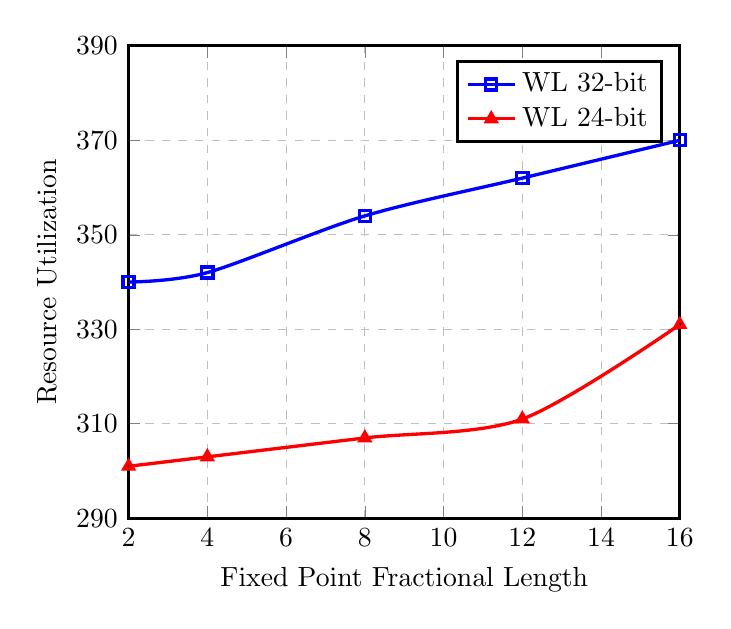
\begin{tikzpicture}
\begin{axis}[
scale only axis,
height=6cm,
width=7cm,
    xlabel={Fixed Point Fractional Length},
    ylabel={Resource Utilization},
    xmin=2, xmax=16,
    ymin=290, ymax=390,
    xtick={2,4,6,8,10,12,14,16},
    ytick={290,310,330,350,370,390},
    legend pos=north east,
    ymajorgrids=true,
    xmajorgrids=true,
    grid style=dashed,
    very thick
]
\addplot[
    color=blue,
    mark=square,
    smooth
    ]
    coordinates {
    (2,340)(4,342)(8,354)(12,362)(16,370)
    };
    \addlegendentry{WL 32-bit}
 \addplot[
    color=red,
    mark=triangle,
    smooth
    ]
    coordinates {
    (2,301)(4,303)(8,307)(12,311)(16,331)
    };
   \addlegendentry{WL 24-bit}
\end{axis}
\end{tikzpicture}
\caption{Effect of varying the Fractional Length on Resource Utilization}
\label{fig:5.5}
\end{figure}
\noindent It was observed that changing the fractional length as well as word length significantly reduces the number of resources used for the computation as can be seen from figure \ref{fig:5.5}.

\begin{figure}[!h]
\centering
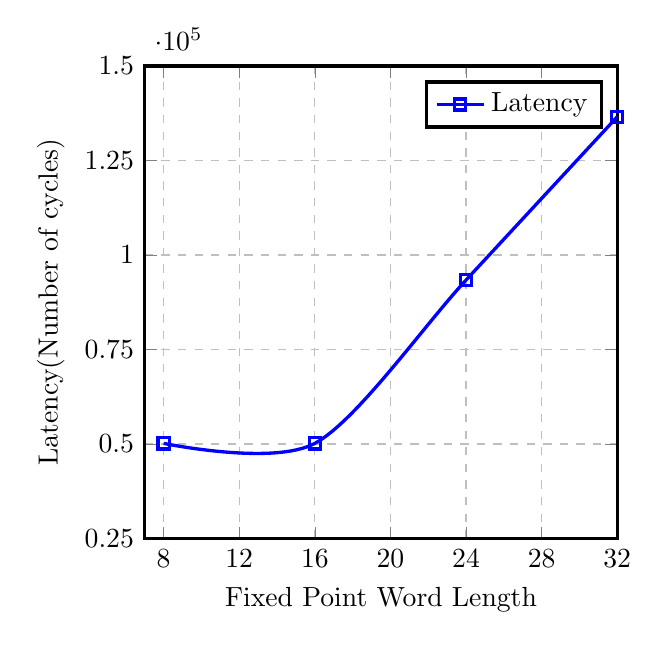
\begin{tikzpicture}
\begin{axis}[
scale only axis,
height=6cm,
width=6cm,
    xlabel={Fixed Point Word Length},
    ylabel={Latency(Number of cycles)},
    xmin=7, xmax=32,
    ymin=25000, ymax=150000,
    xtick={8,12,16,20,24,28,32},
    ytick={25000,50000,75000,100000,125000,150000},
    legend pos=north east,
    ymajorgrids=true,
    xmajorgrids=true,
    grid style=dashed,
    very thick
]
\addplot[
    color=blue,
    mark=square,
    smooth
    ]
    coordinates {
    (32,136562)(24,93362)(16,50162)(8,50162)
    };
    \addlegendentry{Latency}
\end{axis}
\end{tikzpicture}
\caption{Effect of varying the Fixed Point Word Length on Latency}
\label{fig:5.6}
\end{figure}
\noindent It was observed that changing the fractional length for a fixed word length doesn't have any impact on the latency for this algorithm. However the latency is improved by reducing the word length. The effect of varying the word length on the latency is demonstrated in figure \ref{fig:5.6}.

\noindent It should be noted that reducing the word length and fractional length at the same time have an adverse effect on the accuracy of the algorithm. So the trade offs must be analyzed before choosing the Q formats. Similarly changing the arithmetic blindly can affect the correctness of the scheme as is analyzed for FHEW. In the following chapter, the results and conclusions drawn from the experiments are demonstrated. 
\chapter{Conclusions and Future Work}\label{Chapter6}
\section{Conclusions}
Two applications were studied thoroughly for the identification of the compute intensive kernels of the algorithms. 
For FHE, 1024 point double precision FFT was identified as the computationally intense portion to be offloaded to hardware. 
It was observed that the modification from double precision to single precision floating point FFT results in significant loss of accuracy and inaccurate implementation because of errors in computation of FFT.
To proceed with, a bottom up analysis of FPGA based double precision floating point FFT was performed, starting from the implementation of a single butterfly unit. An implementation was achieved which is estimated to compute a 1024-Point FFT in 1.19ms, while consuming a significantly lesser resource utilization.
%An implementation was achieved which uses only one double precision multiplier and one double precision adder-subtractor unit for the entire computation, consuming only 1\% FF's,4\% LUT's and 6\% DSP's on Zedboard ZC702. 

For CNN, convolution was identified as the compute intensive portion and the underlying arithmetic was modified from floating point to fixed point. It was observed that the same accuracy can be obtained if we change the arithmetic from single precision float to Fixed point Q-Combinations of (32,16) or(24-16).
It saves almost 70\% resources as compared to floating point for Q(32-16) combination and further improvement of 8\% in resources can be obtained by using the Q(24-16) format. 
%A speed up of 1.7 is estimated for Q(24.16) format. 

\section{Future Work}
\begin{itemize}
%\item
%\textbf{Real Time Estimation:} The current implementation gives the performance enhancement of the application, for one iteration of the algorithm. However the estimates may be different, in terms of real time streaming of input. e.g. for FHEW library, the results are computed only for one iteration of HOMNAND, however real time circuits might need to execute multiple iterations of NAND, which may lead to more consumption of resources at run time. Bench marking for variable circuit depths is a future work and can be extended for this thesis.
\item \textbf{FHE Optimization:} It was oberved based on analysis that single precision float data type results in significant loss of accuracy, however another method to optimize FHE is by changing the noise variable or modulo factor 'q', such that the FFT can be modified to NTT operation. 
%\item
%\textbf{Streaming:} This report analyses the kernels in an algorithm for offloading to the hardware, their implementation in hardware, and performance estimation based on resource utilization.  Since the entire analysis is to achieve a high degree of parallelism, a suitable interconnect architecture is needed for executing it. The effect of modification of arithmetic on streaming interfaces i.e. when the data is communicated from processor to programmable logic can be the verified as an extension to this work.
%\item \textbf{Accelerator Specific Optimization :} This report analyses one area of accelerator specific optimization i.e. the arithmetic. Other areas of optimization e.g. Integration of accelerators with memory can be explored as future work.

\end{itemize}




%Bibliographic references
\begin{thebibliography}{9}


\bibitem{FHEW} \label{fhew1}
Léo Ducas and Daniele Micciancio,"FHEW: Bootstrapping Homomorphic Encryption in less than a second"
\textit{Cryptology ePrint Archive 2014/816,} 2014.

\bibitem{easyfhe} \label{easyfhe}
Craig Gentry,"Computing Arbitrary Functions of Encrypted Data"
\textit{https://crypto.stanford.edu/craig/easy-fhe.pdf} 

\bibitem{FHEW Library} \label{fhewlib}
L. Ducas and D. Micciancio. Implementation of FHEW.
\textit{https://github.com/lducas/FHEW} June 2014.

\bibitem{FFTW} \label{fftw}
Matteo Frigo and Steven G. Johnson,"Fastest Fourier Transform in the West"
\textit{http://www.fftw.org}.

\bibitem{FFTW_paper} \label{fftw_paper}
Matteo Frigo,"A Fast Fourier Transform Compiler"
\textit{MIT Laboratory for Computer Science}.February 1999.

\bibitem{Libfi} \label{lib}
Gabi Sarkis. 
\textit{https://github.com/gsarkis/libfi}. 

\bibitem{FHEW ideal Lattices} \label{lattices}
Craig Gentry,"Fully Homomorphic Encryption Using Ideal Lattices".
\textit{ In M. Mitzenmacher, editor,41st ACM STOC,pages 169–178. ACM Press} May / June 2009.

\bibitem{FFTW} \label{homo}
Brian Hayes,"Alice and Bob in Cipherspace"
\textit{http://www.americanscientist.org/libraries/documents/201286159329266-2012-09CompSciHayes.pdf}.

\bibitem{FFTW3} \label{FFTW3git}
"FFTW/fftw3"
\textit{https://github.com/FFTW/fftw3.git}.


\bibitem{FFT accuracy}  \label{FFT accuracy}
James C. Schatzman. Accuracy of the Discrete Fourier Transform and the Fast Fourier Transform.
\textit{https://pdfs.semanticscholar.org/9939/893e66a57e89271c5bcd2d64b2a961cf4425.pdf}

\bibitem{Papaa} \label{papaa}
Gopalakrishna Hegde, Nachiappan Ramasamy, Nachiket Kapre.OpenCL Labs for PAPAA Summer School 2016 Edition.
\textit{https://github.com/gplhegde/papaa-opencl}. 

\bibitem{Eli Hughes} 
Eli Hughes. (2014, April 28). Introduction to Fixed Point Math for Embedded Systems [Video File].Retrieved from
\textit{https://www.youtube.com/user/emh203/videos}

\bibitem{Double Precision} \label{dp}
Double-precision floating-point format.
\textit{https://en.wikipedia.org/wiki/Double-precision\_floating-point\_format}

\bibitem{Vivado Design Suite} \label{Vivado}
\textit{Vivado Design Suite User Guide, High-Level Synthesis}

\bibitem{accuracy fftw3} \label{accuracy fftw3}
benchFFT,\textit{http://www.fftw.org/accuracy/}

\bibitem{oppenheim} \label{accuracy fftw3}
Discrete-Time Signal Processing, Alan V. Oppenheim, Ronald W. Schafer,John R. Busk.
\textit{Prentice Hall,New Jeresy} 1998.

\bibitem{architechture} \label{architechture}
Architechture Exploration of FPGA based Accelerators for Bioinformatics Applications, B. Sharat Chandra Varma,Kolin Paul, M. Balakrishnan.
\textit{Springer Series in Advanced Microelectronics,Singapore} 2016.
\end{thebibliography}



%\end{document}






\end{document}
